\begin{enumerate}[label=\thesubsection.\arabic*,ref=\thesubsection.\theenumi]
\item Find the slope of the tangent to the curve $y = \frac{x-1}{x-2}$, $x \neq 2$ at $x=10$.
	\\
\solution 
\label{chapters/12/6/3/2}
\iffalse
\documentclass[journal,10pt,twocolumn]{article}
\usepackage{graphicx, float}
\usepackage[margin=0.5in]{geometry}
\usepackage{amsmath, bm}
\usepackage{array}
\usepackage{booktabs}
\usepackage[utf8]{inputenc}
\usepackage{amsfonts}
\usepackage{amssymb}
\usepackage{graphicx}
\usepackage{multicol}
\usepackage{tabularx}
\usepackage{hyperref}
\usepackage{mathtools}
\DeclareUnicodeCharacter{2212}{-}
\providecommand{\norm}[1]{\left\lVert#1\right\rVert}
\providecommand{\abs}[1]{\left\vert#1\right\vert}
\let\vec\mathbf
\newcommand{\myvec}[1]{\ensuremath{\begin{pmatrix}#1\end{pmatrix}}}
\newcommand{\mydet}[1]{\ensuremath{\begin{vmatrix}#1\end{vmatrix}}}
\providecommand{\brak}[1]{\ensuremath{\left(#1\right)}}
\providecommand{\lbrak}[1]{\ensuremath{\left(#1\right.}}
\providecommand{\rbrak}[1]{\ensuremath{\left.#1\right)}}
\providecommand{\sbrak}[1]{\ensuremath{{}\left[#1\right]}}
%\providecommand{\norm}[1]{\left\lVert#1\right\rVert}
%\providecommand{\sbrak}[1]{\ensuremath{{}\left[#1\right]}}
%\providecommand{\lsbrak}[1]{\ensuremath{{}\left[#1\right.}}
%\providecommand{\rsbrak}[1]{\ensuremath{{}\left.#1\right]}}
%\providecommand{\brak}[1]{\ensuremath{\left(#1\right)}}
%\providecommand{\lbrak}[1]{\ensuremath{\left(#1\right.}}
%\providecommand{\rbrak}[1]{\ensuremath{\left.#1\right)}}
%\providecommand{\cbrak}[1]{\ensuremath{\left\{#1\right\}}}
%\providecommand{\lcbrak}[1]{\ensuremath{\left\{#1\right.}}
%\providecommand{\rcbrak}[1]{\ensuremath{\left.#1\right\}}}
%\newcommand{\myvec}[1]{\ensuremath{\begin{pmatrix}#1\end{pmatrix}}}
%\let\vec\mathbf

\title{\textbf{Conic Assignment}}
\author{Namrath Pinnamaneni \hspace{9cm} FWC22042}
\date{September 2022}

\begin{document}

\maketitle
\paragraph{\textit{Problem Statement} -
\fi
Find the normal to the curve $x_2=4y$ passing (1,2). 
\iffalse
(a)x+y=3  \hspace{2cm} (b)x-y=3\\ 
(c)x+y=1 \hspace{2cm}  (d)x-y=1\\}

\section*{\large Solution}

\begin{figure}[H]
\centering
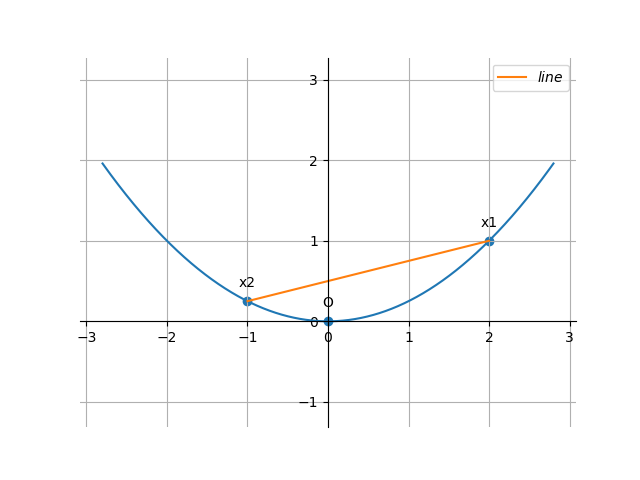
\includegraphics[width=0.75\columnwidth]{conic.png}
\caption{Tangents from A to circle through B, C and D}
\label{fig:triangle}
\end{figure}

The given equation of parabola $x^2 = 4y$ can be written in the general quadratic form as
\begin{align}
    \label{eq:conic_quad_form}
    \vec{x}^{\top}\vec{V}\vec{x}+2\vec{u}^{\top}\vec{x}+f=0
    \end{align}
where
\begin{align}
	\label{eq:V_matrix}
	\vec{V} &= \myvec{1 & 0\\0 & 0},
	\\
	\label{eq:u_vector}
	\vec{u} &= \myvec{0\\-2},
	\\
	\label{eq:f_value}
	f &= 0
	%\\
\end{align}

Let the point from which normals are drawn be $\vec{h}$. Then, the equation of the normal can be written as
\begin{align}
	\vec{x} = \vec{h} + \lambda\vec{m}
	\label{eq:normal_chord}
\end{align}
Say the point of intersection of \eqref{eq:normal_chord} with the conic is $\vec{q}$. A tangent drawn at $\vec{q}$ satisfies the equation
\begin{align}
	\label{eq:tangency_condition}
	\vec{n}^\top(\vec{Vq}+\vec{u}) = 0
\end{align}
Where $\vec{n}$ is the direction vector of the tangent and is perpendicular to $\vec{m}$ in \eqref{eq:normal_chord}.\\\\
In general, the parameter values for points of intersection of a line given by \eqref{eq:normal_chord} with a conic is given by
{\tiny
\begin{multline}
\lambda_i = \frac{1}
{
\vec{m}^T\vec{V}\vec{m}
}
\lbrak{-\vec{m}^T\brak{\vec{V}\vec{h}+\vec{u}}}
\\
\pm
\rbrak{\sqrt{
\sbrak{
\vec{m}^T\brak{\vec{V}\vec{h}+\vec{u}}
}^2
-
\brak
{
\vec{h}^T\vec{V}\vec{h} + 2\vec{u}^T\vec{h} +f
}
\brak{\vec{m}^T\vec{V}\vec{m}}
}
}
\label{eq:tangent_roots}
\end{multline}
}
Using \eqref{eq:tangent_roots} and \eqref{eq:normal_chord}, the intersection point $\vec{q}$ can be written as
\begin{align}
	\label{eq:point_of_tangency}
	\vec{q} = \vec{h} + \lambda_i\vec{m}
\end{align}
Substituting \eqref{eq:point_of_tangency} in \eqref{eq:tangency_condition},
\begin{align}
	\label{eq:normal_simp_1}
	\vec{n}^\top(\vec{V}(\vec{h}+\lambda_i\vec{m})+\vec{u}) = 0\\
	\label{eq:normal_simp_2}
	\implies \lambda_i\vec{n}^\top\vec{V}\vec{m} = -\vec{n}^\top(\vec{Vh}+\vec{u})
\end{align}
Substituting value of $\lambda_i$ from \eqref{eq:tangent_roots} in \eqref{eq:normal_simp_2}
{\tiny
\begin{multline}
	\frac{1}{\vec{m}^\top\vec{V}\vec{m}}\lbrak{-\vec{m}^\top\brak{\vec{Vh}+\vec{u}}} \\ 
	\pm \rbrak{\sqrt{\sbrak{\vec{m}^T\brak{\vec{V}\vec{h}+\vec{u}}}^2-\brak{\vec{h}^T\vec{V}\vec{h} + 2\vec{u}^T\vec{h} +f}\brak{\vec{m}^T\vec{V}\vec{m}}}}\vec{n}^\top\vec{V}\vec{m} \\
	= -\vec{n}^\top\brak{\vec{Vh}+\vec{u}}
	\label{eq:normal_simp_3}
\end{multline}
}
Rearranging the terms,
{\tiny
\begin{multline}
	\pm \sqrt{\sbrak{\vec{m}^T\brak{\vec{V}\vec{h}+\vec{u}}}^2-\brak{\vec{h}^T\vec{V}\vec{h} + 2\vec{u}^T\vec{h} +f}\brak{\vec{m}^T\vec{V}\vec{m}}} \brak{\vec{n}^\top\vec{V}\vec{m}} \\ = \brak{\vec{Vh}+\vec{u}}^\top\brak{\brak{\vec{n}^\top\vec{V}\vec{m}}\vec{m}-\brak{\vec{m}^\top\vec{V}\vec{m}}\vec{n}}
\end{multline}
}
Squaring on both sides
{\tiny
\begin{multline}
	\sbrak{\sbrak{\vec{m}^T\brak{\vec{V}\vec{h}+\vec{u}}}^2-\brak{\vec{h}^T\vec{V}\vec{h} + 2\vec{u}^T\vec{h} +f}\brak{\vec{m}^T\vec{V}\vec{m}}}\brak{\vec{n}^\top\vec{V}\vec{m}}^2 \\ = \sbrak{\brak{\vec{Vh}+\vec{u}}^\top\brak{\brak{\vec{n}^\top\vec{V}\vec{m}}\vec{m}-\brak{\vec{m}^\top\vec{V}\vec{m}}\vec{n}}}^2
	\label{eq:normal_solution}
\end{multline}
}\\
If $\vec{n}$ is taken as $\myvec{-\mu \\ 1}$, then $\vec{m}$ is $\myvec{-1 \\ -\mu}$. Substituting these values in \eqref{eq:normal_solution} and solving for $\mu$, the different possible normals passing through $\vec{h}$ are obtained.\\\\
Thus after solving we get the following values for $\mu$ = {-1, 1/2 - sqrt(3)*I/2, 1/2 + sqrt(3)*I/2}\\\\
Taking $\mu$=1 we get,
\begin{center}
$\vec{n} = \myvec{1 \\ 1}$, $\vec{m} = \myvec{-1 \\ 1}$\\
\end{center}
By calculating $\lambda_i$ from \eqref{eq:normal_simp_2}, we get
\begin{center}
    $\lambda_i = -1$
\end{center}
We find out $\vec{q}$ from \eqref{eq:point_of_tangency},
\begin{center}
where $\vec{h} = \myvec{1 \\ 2}$, $\vec{m} = \myvec{-1 \\ 1}$, $\lambda_i = -1$
\end{center}
\begin{center}
    $\vec{q} = \myvec{1 \\ 2} + (-1)\myvec{-1 \\ 1} = $\myvec{2 \\ 1}
\end{center}
\begin{center}
    Thus $\vec{q}$ satisfies Option(a) i.e. $x+y=3$
\end{center} 

\section*{\large Construction}
{
\setlength\extrarowheight{5pt}
\begin{tabular}{|c|c|c|}
	\hline
	\textbf{Symbol}&\textbf{Value}&\textbf{Description}\\[5pt]
	\hline
	$\vec{h}$&$\myvec{1 \\ 2}$&Given point through which Normal is passing\\[5pt]
	\hline
	$\vec{q}$&$\myvec{2 \\ 1}$&Foot of Normal\\[5pt]
	\hline
	$\vec{m}$ & $\myvec{-1 \\ 1}$ & Direction Vector of Normal\\[5pt]
	\hline
	$\vec{n}$ & $\myvec{1 \\ 1}$ & Direction Vector of Tangent at $\myvec{q}$\\
	\hline
\end{tabular}
}

\end{document}
\fi

\item 
		Find a point on the curve \begin{align}y=(x-2)^2\end{align} at which a tangent is parallel to the chord joining the points (2,0) and (4,4).
			\\
			\solution 
\label{chapters/12/6/3/8}
\iffalse
\documentclass[journal,10pt,twocolumn]{article}
\usepackage{graphicx, float}
\usepackage[margin=0.5in]{geometry}
\usepackage{amsmath, bm}
\usepackage{array}
\usepackage{booktabs}
\usepackage[utf8]{inputenc}
\usepackage{amsfonts}
\usepackage{amssymb}
\usepackage{graphicx}
\usepackage{multicol}
\usepackage{tabularx}
\usepackage{hyperref}
\usepackage{mathtools}
\DeclareUnicodeCharacter{2212}{-}
\providecommand{\norm}[1]{\left\lVert#1\right\rVert}
\providecommand{\abs}[1]{\left\vert#1\right\vert}
\let\vec\mathbf
\newcommand{\myvec}[1]{\ensuremath{\begin{pmatrix}#1\end{pmatrix}}}
\newcommand{\mydet}[1]{\ensuremath{\begin{vmatrix}#1\end{vmatrix}}}
\providecommand{\brak}[1]{\ensuremath{\left(#1\right)}}
\providecommand{\lbrak}[1]{\ensuremath{\left(#1\right.}}
\providecommand{\rbrak}[1]{\ensuremath{\left.#1\right)}}
\providecommand{\sbrak}[1]{\ensuremath{{}\left[#1\right]}}
%\providecommand{\norm}[1]{\left\lVert#1\right\rVert}
%\providecommand{\sbrak}[1]{\ensuremath{{}\left[#1\right]}}
%\providecommand{\lsbrak}[1]{\ensuremath{{}\left[#1\right.}}
%\providecommand{\rsbrak}[1]{\ensuremath{{}\left.#1\right]}}
%\providecommand{\brak}[1]{\ensuremath{\left(#1\right)}}
%\providecommand{\lbrak}[1]{\ensuremath{\left(#1\right.}}
%\providecommand{\rbrak}[1]{\ensuremath{\left.#1\right)}}
%\providecommand{\cbrak}[1]{\ensuremath{\left\{#1\right\}}}
%\providecommand{\lcbrak}[1]{\ensuremath{\left\{#1\right.}}
%\providecommand{\rcbrak}[1]{\ensuremath{\left.#1\right\}}}
%\newcommand{\myvec}[1]{\ensuremath{\begin{pmatrix}#1\end{pmatrix}}}
%\let\vec\mathbf

\title{\textbf{Conic Assignment}}
\author{Namrath Pinnamaneni \hspace{9cm} FWC22042}
\date{September 2022}

\begin{document}

\maketitle
\paragraph{\textit{Problem Statement} -
\fi
Find the normal to the curve $x_2=4y$ passing (1,2). 
\iffalse
(a)x+y=3  \hspace{2cm} (b)x-y=3\\ 
(c)x+y=1 \hspace{2cm}  (d)x-y=1\\}

\section*{\large Solution}

\begin{figure}[H]
\centering
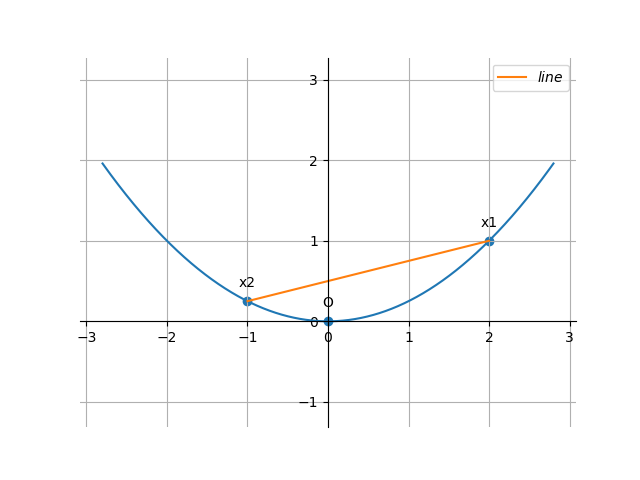
\includegraphics[width=0.75\columnwidth]{conic.png}
\caption{Tangents from A to circle through B, C and D}
\label{fig:triangle}
\end{figure}

The given equation of parabola $x^2 = 4y$ can be written in the general quadratic form as
\begin{align}
    \label{eq:conic_quad_form}
    \vec{x}^{\top}\vec{V}\vec{x}+2\vec{u}^{\top}\vec{x}+f=0
    \end{align}
where
\begin{align}
	\label{eq:V_matrix}
	\vec{V} &= \myvec{1 & 0\\0 & 0},
	\\
	\label{eq:u_vector}
	\vec{u} &= \myvec{0\\-2},
	\\
	\label{eq:f_value}
	f &= 0
	%\\
\end{align}

Let the point from which normals are drawn be $\vec{h}$. Then, the equation of the normal can be written as
\begin{align}
	\vec{x} = \vec{h} + \lambda\vec{m}
	\label{eq:normal_chord}
\end{align}
Say the point of intersection of \eqref{eq:normal_chord} with the conic is $\vec{q}$. A tangent drawn at $\vec{q}$ satisfies the equation
\begin{align}
	\label{eq:tangency_condition}
	\vec{n}^\top(\vec{Vq}+\vec{u}) = 0
\end{align}
Where $\vec{n}$ is the direction vector of the tangent and is perpendicular to $\vec{m}$ in \eqref{eq:normal_chord}.\\\\
In general, the parameter values for points of intersection of a line given by \eqref{eq:normal_chord} with a conic is given by
{\tiny
\begin{multline}
\lambda_i = \frac{1}
{
\vec{m}^T\vec{V}\vec{m}
}
\lbrak{-\vec{m}^T\brak{\vec{V}\vec{h}+\vec{u}}}
\\
\pm
\rbrak{\sqrt{
\sbrak{
\vec{m}^T\brak{\vec{V}\vec{h}+\vec{u}}
}^2
-
\brak
{
\vec{h}^T\vec{V}\vec{h} + 2\vec{u}^T\vec{h} +f
}
\brak{\vec{m}^T\vec{V}\vec{m}}
}
}
\label{eq:tangent_roots}
\end{multline}
}
Using \eqref{eq:tangent_roots} and \eqref{eq:normal_chord}, the intersection point $\vec{q}$ can be written as
\begin{align}
	\label{eq:point_of_tangency}
	\vec{q} = \vec{h} + \lambda_i\vec{m}
\end{align}
Substituting \eqref{eq:point_of_tangency} in \eqref{eq:tangency_condition},
\begin{align}
	\label{eq:normal_simp_1}
	\vec{n}^\top(\vec{V}(\vec{h}+\lambda_i\vec{m})+\vec{u}) = 0\\
	\label{eq:normal_simp_2}
	\implies \lambda_i\vec{n}^\top\vec{V}\vec{m} = -\vec{n}^\top(\vec{Vh}+\vec{u})
\end{align}
Substituting value of $\lambda_i$ from \eqref{eq:tangent_roots} in \eqref{eq:normal_simp_2}
{\tiny
\begin{multline}
	\frac{1}{\vec{m}^\top\vec{V}\vec{m}}\lbrak{-\vec{m}^\top\brak{\vec{Vh}+\vec{u}}} \\ 
	\pm \rbrak{\sqrt{\sbrak{\vec{m}^T\brak{\vec{V}\vec{h}+\vec{u}}}^2-\brak{\vec{h}^T\vec{V}\vec{h} + 2\vec{u}^T\vec{h} +f}\brak{\vec{m}^T\vec{V}\vec{m}}}}\vec{n}^\top\vec{V}\vec{m} \\
	= -\vec{n}^\top\brak{\vec{Vh}+\vec{u}}
	\label{eq:normal_simp_3}
\end{multline}
}
Rearranging the terms,
{\tiny
\begin{multline}
	\pm \sqrt{\sbrak{\vec{m}^T\brak{\vec{V}\vec{h}+\vec{u}}}^2-\brak{\vec{h}^T\vec{V}\vec{h} + 2\vec{u}^T\vec{h} +f}\brak{\vec{m}^T\vec{V}\vec{m}}} \brak{\vec{n}^\top\vec{V}\vec{m}} \\ = \brak{\vec{Vh}+\vec{u}}^\top\brak{\brak{\vec{n}^\top\vec{V}\vec{m}}\vec{m}-\brak{\vec{m}^\top\vec{V}\vec{m}}\vec{n}}
\end{multline}
}
Squaring on both sides
{\tiny
\begin{multline}
	\sbrak{\sbrak{\vec{m}^T\brak{\vec{V}\vec{h}+\vec{u}}}^2-\brak{\vec{h}^T\vec{V}\vec{h} + 2\vec{u}^T\vec{h} +f}\brak{\vec{m}^T\vec{V}\vec{m}}}\brak{\vec{n}^\top\vec{V}\vec{m}}^2 \\ = \sbrak{\brak{\vec{Vh}+\vec{u}}^\top\brak{\brak{\vec{n}^\top\vec{V}\vec{m}}\vec{m}-\brak{\vec{m}^\top\vec{V}\vec{m}}\vec{n}}}^2
	\label{eq:normal_solution}
\end{multline}
}\\
If $\vec{n}$ is taken as $\myvec{-\mu \\ 1}$, then $\vec{m}$ is $\myvec{-1 \\ -\mu}$. Substituting these values in \eqref{eq:normal_solution} and solving for $\mu$, the different possible normals passing through $\vec{h}$ are obtained.\\\\
Thus after solving we get the following values for $\mu$ = {-1, 1/2 - sqrt(3)*I/2, 1/2 + sqrt(3)*I/2}\\\\
Taking $\mu$=1 we get,
\begin{center}
$\vec{n} = \myvec{1 \\ 1}$, $\vec{m} = \myvec{-1 \\ 1}$\\
\end{center}
By calculating $\lambda_i$ from \eqref{eq:normal_simp_2}, we get
\begin{center}
    $\lambda_i = -1$
\end{center}
We find out $\vec{q}$ from \eqref{eq:point_of_tangency},
\begin{center}
where $\vec{h} = \myvec{1 \\ 2}$, $\vec{m} = \myvec{-1 \\ 1}$, $\lambda_i = -1$
\end{center}
\begin{center}
    $\vec{q} = \myvec{1 \\ 2} + (-1)\myvec{-1 \\ 1} = $\myvec{2 \\ 1}
\end{center}
\begin{center}
    Thus $\vec{q}$ satisfies Option(a) i.e. $x+y=3$
\end{center} 

\section*{\large Construction}
{
\setlength\extrarowheight{5pt}
\begin{tabular}{|c|c|c|}
	\hline
	\textbf{Symbol}&\textbf{Value}&\textbf{Description}\\[5pt]
	\hline
	$\vec{h}$&$\myvec{1 \\ 2}$&Given point through which Normal is passing\\[5pt]
	\hline
	$\vec{q}$&$\myvec{2 \\ 1}$&Foot of Normal\\[5pt]
	\hline
	$\vec{m}$ & $\myvec{-1 \\ 1}$ & Direction Vector of Normal\\[5pt]
	\hline
	$\vec{n}$ & $\myvec{1 \\ 1}$ & Direction Vector of Tangent at $\myvec{q}$\\
	\hline
\end{tabular}
}

\end{document}
\fi

\item 
Find the equation of all lines having slope  -1 that are tangents to the curve
\begin{align}
y = \frac{1}{x-1}, x \neq 1
\label{chapters/12/6/3/10}
\end{align}
	\\
	\solution 
\iffalse
\documentclass[journal,10pt,twocolumn]{article}
\usepackage{graphicx, float}
\usepackage[margin=0.5in]{geometry}
\usepackage{amsmath, bm}
\usepackage{array}
\usepackage{booktabs}
\usepackage[utf8]{inputenc}
\usepackage{amsfonts}
\usepackage{amssymb}
\usepackage{graphicx}
\usepackage{multicol}
\usepackage{tabularx}
\usepackage{hyperref}
\usepackage{mathtools}
\DeclareUnicodeCharacter{2212}{-}
\providecommand{\norm}[1]{\left\lVert#1\right\rVert}
\providecommand{\abs}[1]{\left\vert#1\right\vert}
\let\vec\mathbf
\newcommand{\myvec}[1]{\ensuremath{\begin{pmatrix}#1\end{pmatrix}}}
\newcommand{\mydet}[1]{\ensuremath{\begin{vmatrix}#1\end{vmatrix}}}
\providecommand{\brak}[1]{\ensuremath{\left(#1\right)}}
\providecommand{\lbrak}[1]{\ensuremath{\left(#1\right.}}
\providecommand{\rbrak}[1]{\ensuremath{\left.#1\right)}}
\providecommand{\sbrak}[1]{\ensuremath{{}\left[#1\right]}}
%\providecommand{\norm}[1]{\left\lVert#1\right\rVert}
%\providecommand{\sbrak}[1]{\ensuremath{{}\left[#1\right]}}
%\providecommand{\lsbrak}[1]{\ensuremath{{}\left[#1\right.}}
%\providecommand{\rsbrak}[1]{\ensuremath{{}\left.#1\right]}}
%\providecommand{\brak}[1]{\ensuremath{\left(#1\right)}}
%\providecommand{\lbrak}[1]{\ensuremath{\left(#1\right.}}
%\providecommand{\rbrak}[1]{\ensuremath{\left.#1\right)}}
%\providecommand{\cbrak}[1]{\ensuremath{\left\{#1\right\}}}
%\providecommand{\lcbrak}[1]{\ensuremath{\left\{#1\right.}}
%\providecommand{\rcbrak}[1]{\ensuremath{\left.#1\right\}}}
%\newcommand{\myvec}[1]{\ensuremath{\begin{pmatrix}#1\end{pmatrix}}}
%\let\vec\mathbf

\title{\textbf{Conic Assignment}}
\author{Namrath Pinnamaneni \hspace{9cm} FWC22042}
\date{September 2022}

\begin{document}

\maketitle
\paragraph{\textit{Problem Statement} -
\fi
Find the normal to the curve $x_2=4y$ passing (1,2). 
\iffalse
(a)x+y=3  \hspace{2cm} (b)x-y=3\\ 
(c)x+y=1 \hspace{2cm}  (d)x-y=1\\}

\section*{\large Solution}

\begin{figure}[H]
\centering
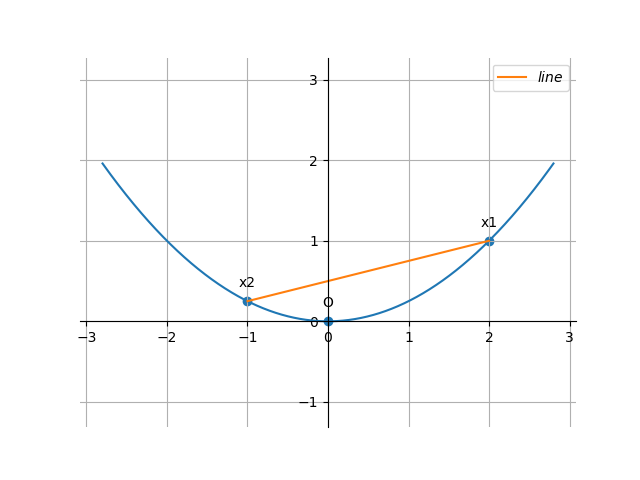
\includegraphics[width=0.75\columnwidth]{conic.png}
\caption{Tangents from A to circle through B, C and D}
\label{fig:triangle}
\end{figure}

The given equation of parabola $x^2 = 4y$ can be written in the general quadratic form as
\begin{align}
    \label{eq:conic_quad_form}
    \vec{x}^{\top}\vec{V}\vec{x}+2\vec{u}^{\top}\vec{x}+f=0
    \end{align}
where
\begin{align}
	\label{eq:V_matrix}
	\vec{V} &= \myvec{1 & 0\\0 & 0},
	\\
	\label{eq:u_vector}
	\vec{u} &= \myvec{0\\-2},
	\\
	\label{eq:f_value}
	f &= 0
	%\\
\end{align}

Let the point from which normals are drawn be $\vec{h}$. Then, the equation of the normal can be written as
\begin{align}
	\vec{x} = \vec{h} + \lambda\vec{m}
	\label{eq:normal_chord}
\end{align}
Say the point of intersection of \eqref{eq:normal_chord} with the conic is $\vec{q}$. A tangent drawn at $\vec{q}$ satisfies the equation
\begin{align}
	\label{eq:tangency_condition}
	\vec{n}^\top(\vec{Vq}+\vec{u}) = 0
\end{align}
Where $\vec{n}$ is the direction vector of the tangent and is perpendicular to $\vec{m}$ in \eqref{eq:normal_chord}.\\\\
In general, the parameter values for points of intersection of a line given by \eqref{eq:normal_chord} with a conic is given by
{\tiny
\begin{multline}
\lambda_i = \frac{1}
{
\vec{m}^T\vec{V}\vec{m}
}
\lbrak{-\vec{m}^T\brak{\vec{V}\vec{h}+\vec{u}}}
\\
\pm
\rbrak{\sqrt{
\sbrak{
\vec{m}^T\brak{\vec{V}\vec{h}+\vec{u}}
}^2
-
\brak
{
\vec{h}^T\vec{V}\vec{h} + 2\vec{u}^T\vec{h} +f
}
\brak{\vec{m}^T\vec{V}\vec{m}}
}
}
\label{eq:tangent_roots}
\end{multline}
}
Using \eqref{eq:tangent_roots} and \eqref{eq:normal_chord}, the intersection point $\vec{q}$ can be written as
\begin{align}
	\label{eq:point_of_tangency}
	\vec{q} = \vec{h} + \lambda_i\vec{m}
\end{align}
Substituting \eqref{eq:point_of_tangency} in \eqref{eq:tangency_condition},
\begin{align}
	\label{eq:normal_simp_1}
	\vec{n}^\top(\vec{V}(\vec{h}+\lambda_i\vec{m})+\vec{u}) = 0\\
	\label{eq:normal_simp_2}
	\implies \lambda_i\vec{n}^\top\vec{V}\vec{m} = -\vec{n}^\top(\vec{Vh}+\vec{u})
\end{align}
Substituting value of $\lambda_i$ from \eqref{eq:tangent_roots} in \eqref{eq:normal_simp_2}
{\tiny
\begin{multline}
	\frac{1}{\vec{m}^\top\vec{V}\vec{m}}\lbrak{-\vec{m}^\top\brak{\vec{Vh}+\vec{u}}} \\ 
	\pm \rbrak{\sqrt{\sbrak{\vec{m}^T\brak{\vec{V}\vec{h}+\vec{u}}}^2-\brak{\vec{h}^T\vec{V}\vec{h} + 2\vec{u}^T\vec{h} +f}\brak{\vec{m}^T\vec{V}\vec{m}}}}\vec{n}^\top\vec{V}\vec{m} \\
	= -\vec{n}^\top\brak{\vec{Vh}+\vec{u}}
	\label{eq:normal_simp_3}
\end{multline}
}
Rearranging the terms,
{\tiny
\begin{multline}
	\pm \sqrt{\sbrak{\vec{m}^T\brak{\vec{V}\vec{h}+\vec{u}}}^2-\brak{\vec{h}^T\vec{V}\vec{h} + 2\vec{u}^T\vec{h} +f}\brak{\vec{m}^T\vec{V}\vec{m}}} \brak{\vec{n}^\top\vec{V}\vec{m}} \\ = \brak{\vec{Vh}+\vec{u}}^\top\brak{\brak{\vec{n}^\top\vec{V}\vec{m}}\vec{m}-\brak{\vec{m}^\top\vec{V}\vec{m}}\vec{n}}
\end{multline}
}
Squaring on both sides
{\tiny
\begin{multline}
	\sbrak{\sbrak{\vec{m}^T\brak{\vec{V}\vec{h}+\vec{u}}}^2-\brak{\vec{h}^T\vec{V}\vec{h} + 2\vec{u}^T\vec{h} +f}\brak{\vec{m}^T\vec{V}\vec{m}}}\brak{\vec{n}^\top\vec{V}\vec{m}}^2 \\ = \sbrak{\brak{\vec{Vh}+\vec{u}}^\top\brak{\brak{\vec{n}^\top\vec{V}\vec{m}}\vec{m}-\brak{\vec{m}^\top\vec{V}\vec{m}}\vec{n}}}^2
	\label{eq:normal_solution}
\end{multline}
}\\
If $\vec{n}$ is taken as $\myvec{-\mu \\ 1}$, then $\vec{m}$ is $\myvec{-1 \\ -\mu}$. Substituting these values in \eqref{eq:normal_solution} and solving for $\mu$, the different possible normals passing through $\vec{h}$ are obtained.\\\\
Thus after solving we get the following values for $\mu$ = {-1, 1/2 - sqrt(3)*I/2, 1/2 + sqrt(3)*I/2}\\\\
Taking $\mu$=1 we get,
\begin{center}
$\vec{n} = \myvec{1 \\ 1}$, $\vec{m} = \myvec{-1 \\ 1}$\\
\end{center}
By calculating $\lambda_i$ from \eqref{eq:normal_simp_2}, we get
\begin{center}
    $\lambda_i = -1$
\end{center}
We find out $\vec{q}$ from \eqref{eq:point_of_tangency},
\begin{center}
where $\vec{h} = \myvec{1 \\ 2}$, $\vec{m} = \myvec{-1 \\ 1}$, $\lambda_i = -1$
\end{center}
\begin{center}
    $\vec{q} = \myvec{1 \\ 2} + (-1)\myvec{-1 \\ 1} = $\myvec{2 \\ 1}
\end{center}
\begin{center}
    Thus $\vec{q}$ satisfies Option(a) i.e. $x+y=3$
\end{center} 

\section*{\large Construction}
{
\setlength\extrarowheight{5pt}
\begin{tabular}{|c|c|c|}
	\hline
	\textbf{Symbol}&\textbf{Value}&\textbf{Description}\\[5pt]
	\hline
	$\vec{h}$&$\myvec{1 \\ 2}$&Given point through which Normal is passing\\[5pt]
	\hline
	$\vec{q}$&$\myvec{2 \\ 1}$&Foot of Normal\\[5pt]
	\hline
	$\vec{m}$ & $\myvec{-1 \\ 1}$ & Direction Vector of Normal\\[5pt]
	\hline
	$\vec{n}$ & $\myvec{1 \\ 1}$ & Direction Vector of Tangent at $\myvec{q}$\\
	\hline
\end{tabular}
}

\end{document}
\fi

\item 
Find the equation of all lines having slope 2 which are tangents to the curve 
\begin{align}
y=\frac{1}{x-3}, x\neq{3} 
\end{align}
\solution 
\label{chapters/12/6/3/11}
\iffalse
\documentclass[journal,10pt,twocolumn]{article}
\usepackage{graphicx, float}
\usepackage[margin=0.5in]{geometry}
\usepackage{amsmath, bm}
\usepackage{array}
\usepackage{booktabs}
\usepackage[utf8]{inputenc}
\usepackage{amsfonts}
\usepackage{amssymb}
\usepackage{graphicx}
\usepackage{multicol}
\usepackage{tabularx}
\usepackage{hyperref}
\usepackage{mathtools}
\DeclareUnicodeCharacter{2212}{-}
\providecommand{\norm}[1]{\left\lVert#1\right\rVert}
\providecommand{\abs}[1]{\left\vert#1\right\vert}
\let\vec\mathbf
\newcommand{\myvec}[1]{\ensuremath{\begin{pmatrix}#1\end{pmatrix}}}
\newcommand{\mydet}[1]{\ensuremath{\begin{vmatrix}#1\end{vmatrix}}}
\providecommand{\brak}[1]{\ensuremath{\left(#1\right)}}
\providecommand{\lbrak}[1]{\ensuremath{\left(#1\right.}}
\providecommand{\rbrak}[1]{\ensuremath{\left.#1\right)}}
\providecommand{\sbrak}[1]{\ensuremath{{}\left[#1\right]}}
%\providecommand{\norm}[1]{\left\lVert#1\right\rVert}
%\providecommand{\sbrak}[1]{\ensuremath{{}\left[#1\right]}}
%\providecommand{\lsbrak}[1]{\ensuremath{{}\left[#1\right.}}
%\providecommand{\rsbrak}[1]{\ensuremath{{}\left.#1\right]}}
%\providecommand{\brak}[1]{\ensuremath{\left(#1\right)}}
%\providecommand{\lbrak}[1]{\ensuremath{\left(#1\right.}}
%\providecommand{\rbrak}[1]{\ensuremath{\left.#1\right)}}
%\providecommand{\cbrak}[1]{\ensuremath{\left\{#1\right\}}}
%\providecommand{\lcbrak}[1]{\ensuremath{\left\{#1\right.}}
%\providecommand{\rcbrak}[1]{\ensuremath{\left.#1\right\}}}
%\newcommand{\myvec}[1]{\ensuremath{\begin{pmatrix}#1\end{pmatrix}}}
%\let\vec\mathbf

\title{\textbf{Conic Assignment}}
\author{Namrath Pinnamaneni \hspace{9cm} FWC22042}
\date{September 2022}

\begin{document}

\maketitle
\paragraph{\textit{Problem Statement} -
\fi
Find the normal to the curve $x_2=4y$ passing (1,2). 
\iffalse
(a)x+y=3  \hspace{2cm} (b)x-y=3\\ 
(c)x+y=1 \hspace{2cm}  (d)x-y=1\\}

\section*{\large Solution}

\begin{figure}[H]
\centering
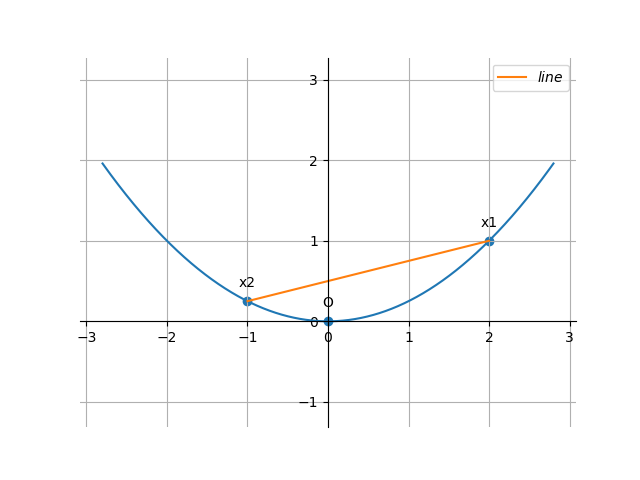
\includegraphics[width=0.75\columnwidth]{conic.png}
\caption{Tangents from A to circle through B, C and D}
\label{fig:triangle}
\end{figure}

The given equation of parabola $x^2 = 4y$ can be written in the general quadratic form as
\begin{align}
    \label{eq:conic_quad_form}
    \vec{x}^{\top}\vec{V}\vec{x}+2\vec{u}^{\top}\vec{x}+f=0
    \end{align}
where
\begin{align}
	\label{eq:V_matrix}
	\vec{V} &= \myvec{1 & 0\\0 & 0},
	\\
	\label{eq:u_vector}
	\vec{u} &= \myvec{0\\-2},
	\\
	\label{eq:f_value}
	f &= 0
	%\\
\end{align}

Let the point from which normals are drawn be $\vec{h}$. Then, the equation of the normal can be written as
\begin{align}
	\vec{x} = \vec{h} + \lambda\vec{m}
	\label{eq:normal_chord}
\end{align}
Say the point of intersection of \eqref{eq:normal_chord} with the conic is $\vec{q}$. A tangent drawn at $\vec{q}$ satisfies the equation
\begin{align}
	\label{eq:tangency_condition}
	\vec{n}^\top(\vec{Vq}+\vec{u}) = 0
\end{align}
Where $\vec{n}$ is the direction vector of the tangent and is perpendicular to $\vec{m}$ in \eqref{eq:normal_chord}.\\\\
In general, the parameter values for points of intersection of a line given by \eqref{eq:normal_chord} with a conic is given by
{\tiny
\begin{multline}
\lambda_i = \frac{1}
{
\vec{m}^T\vec{V}\vec{m}
}
\lbrak{-\vec{m}^T\brak{\vec{V}\vec{h}+\vec{u}}}
\\
\pm
\rbrak{\sqrt{
\sbrak{
\vec{m}^T\brak{\vec{V}\vec{h}+\vec{u}}
}^2
-
\brak
{
\vec{h}^T\vec{V}\vec{h} + 2\vec{u}^T\vec{h} +f
}
\brak{\vec{m}^T\vec{V}\vec{m}}
}
}
\label{eq:tangent_roots}
\end{multline}
}
Using \eqref{eq:tangent_roots} and \eqref{eq:normal_chord}, the intersection point $\vec{q}$ can be written as
\begin{align}
	\label{eq:point_of_tangency}
	\vec{q} = \vec{h} + \lambda_i\vec{m}
\end{align}
Substituting \eqref{eq:point_of_tangency} in \eqref{eq:tangency_condition},
\begin{align}
	\label{eq:normal_simp_1}
	\vec{n}^\top(\vec{V}(\vec{h}+\lambda_i\vec{m})+\vec{u}) = 0\\
	\label{eq:normal_simp_2}
	\implies \lambda_i\vec{n}^\top\vec{V}\vec{m} = -\vec{n}^\top(\vec{Vh}+\vec{u})
\end{align}
Substituting value of $\lambda_i$ from \eqref{eq:tangent_roots} in \eqref{eq:normal_simp_2}
{\tiny
\begin{multline}
	\frac{1}{\vec{m}^\top\vec{V}\vec{m}}\lbrak{-\vec{m}^\top\brak{\vec{Vh}+\vec{u}}} \\ 
	\pm \rbrak{\sqrt{\sbrak{\vec{m}^T\brak{\vec{V}\vec{h}+\vec{u}}}^2-\brak{\vec{h}^T\vec{V}\vec{h} + 2\vec{u}^T\vec{h} +f}\brak{\vec{m}^T\vec{V}\vec{m}}}}\vec{n}^\top\vec{V}\vec{m} \\
	= -\vec{n}^\top\brak{\vec{Vh}+\vec{u}}
	\label{eq:normal_simp_3}
\end{multline}
}
Rearranging the terms,
{\tiny
\begin{multline}
	\pm \sqrt{\sbrak{\vec{m}^T\brak{\vec{V}\vec{h}+\vec{u}}}^2-\brak{\vec{h}^T\vec{V}\vec{h} + 2\vec{u}^T\vec{h} +f}\brak{\vec{m}^T\vec{V}\vec{m}}} \brak{\vec{n}^\top\vec{V}\vec{m}} \\ = \brak{\vec{Vh}+\vec{u}}^\top\brak{\brak{\vec{n}^\top\vec{V}\vec{m}}\vec{m}-\brak{\vec{m}^\top\vec{V}\vec{m}}\vec{n}}
\end{multline}
}
Squaring on both sides
{\tiny
\begin{multline}
	\sbrak{\sbrak{\vec{m}^T\brak{\vec{V}\vec{h}+\vec{u}}}^2-\brak{\vec{h}^T\vec{V}\vec{h} + 2\vec{u}^T\vec{h} +f}\brak{\vec{m}^T\vec{V}\vec{m}}}\brak{\vec{n}^\top\vec{V}\vec{m}}^2 \\ = \sbrak{\brak{\vec{Vh}+\vec{u}}^\top\brak{\brak{\vec{n}^\top\vec{V}\vec{m}}\vec{m}-\brak{\vec{m}^\top\vec{V}\vec{m}}\vec{n}}}^2
	\label{eq:normal_solution}
\end{multline}
}\\
If $\vec{n}$ is taken as $\myvec{-\mu \\ 1}$, then $\vec{m}$ is $\myvec{-1 \\ -\mu}$. Substituting these values in \eqref{eq:normal_solution} and solving for $\mu$, the different possible normals passing through $\vec{h}$ are obtained.\\\\
Thus after solving we get the following values for $\mu$ = {-1, 1/2 - sqrt(3)*I/2, 1/2 + sqrt(3)*I/2}\\\\
Taking $\mu$=1 we get,
\begin{center}
$\vec{n} = \myvec{1 \\ 1}$, $\vec{m} = \myvec{-1 \\ 1}$\\
\end{center}
By calculating $\lambda_i$ from \eqref{eq:normal_simp_2}, we get
\begin{center}
    $\lambda_i = -1$
\end{center}
We find out $\vec{q}$ from \eqref{eq:point_of_tangency},
\begin{center}
where $\vec{h} = \myvec{1 \\ 2}$, $\vec{m} = \myvec{-1 \\ 1}$, $\lambda_i = -1$
\end{center}
\begin{center}
    $\vec{q} = \myvec{1 \\ 2} + (-1)\myvec{-1 \\ 1} = $\myvec{2 \\ 1}
\end{center}
\begin{center}
    Thus $\vec{q}$ satisfies Option(a) i.e. $x+y=3$
\end{center} 

\section*{\large Construction}
{
\setlength\extrarowheight{5pt}
\begin{tabular}{|c|c|c|}
	\hline
	\textbf{Symbol}&\textbf{Value}&\textbf{Description}\\[5pt]
	\hline
	$\vec{h}$&$\myvec{1 \\ 2}$&Given point through which Normal is passing\\[5pt]
	\hline
	$\vec{q}$&$\myvec{2 \\ 1}$&Foot of Normal\\[5pt]
	\hline
	$\vec{m}$ & $\myvec{-1 \\ 1}$ & Direction Vector of Normal\\[5pt]
	\hline
	$\vec{n}$ & $\myvec{1 \\ 1}$ & Direction Vector of Tangent at $\myvec{q}$\\
	\hline
\end{tabular}
}

\end{document}
\fi

\item 
 Find points on the curve $\frac{x^2}{9}+\frac{y^2}{16}=1$ at which the tangents are 
 \begin{enumerate}
	 \item parallel to x-axis\\  
	 \item parallel to y-axis
 \end{enumerate}
 \solution 
\label{chapters/12/6/3/13}
\iffalse
\documentclass[journal,10pt,twocolumn]{article}
\usepackage{graphicx, float}
\usepackage[margin=0.5in]{geometry}
\usepackage{amsmath, bm}
\usepackage{array}
\usepackage{booktabs}
\usepackage[utf8]{inputenc}
\usepackage{amsfonts}
\usepackage{amssymb}
\usepackage{graphicx}
\usepackage{multicol}
\usepackage{tabularx}
\usepackage{hyperref}
\usepackage{mathtools}
\DeclareUnicodeCharacter{2212}{-}
\providecommand{\norm}[1]{\left\lVert#1\right\rVert}
\providecommand{\abs}[1]{\left\vert#1\right\vert}
\let\vec\mathbf
\newcommand{\myvec}[1]{\ensuremath{\begin{pmatrix}#1\end{pmatrix}}}
\newcommand{\mydet}[1]{\ensuremath{\begin{vmatrix}#1\end{vmatrix}}}
\providecommand{\brak}[1]{\ensuremath{\left(#1\right)}}
\providecommand{\lbrak}[1]{\ensuremath{\left(#1\right.}}
\providecommand{\rbrak}[1]{\ensuremath{\left.#1\right)}}
\providecommand{\sbrak}[1]{\ensuremath{{}\left[#1\right]}}
%\providecommand{\norm}[1]{\left\lVert#1\right\rVert}
%\providecommand{\sbrak}[1]{\ensuremath{{}\left[#1\right]}}
%\providecommand{\lsbrak}[1]{\ensuremath{{}\left[#1\right.}}
%\providecommand{\rsbrak}[1]{\ensuremath{{}\left.#1\right]}}
%\providecommand{\brak}[1]{\ensuremath{\left(#1\right)}}
%\providecommand{\lbrak}[1]{\ensuremath{\left(#1\right.}}
%\providecommand{\rbrak}[1]{\ensuremath{\left.#1\right)}}
%\providecommand{\cbrak}[1]{\ensuremath{\left\{#1\right\}}}
%\providecommand{\lcbrak}[1]{\ensuremath{\left\{#1\right.}}
%\providecommand{\rcbrak}[1]{\ensuremath{\left.#1\right\}}}
%\newcommand{\myvec}[1]{\ensuremath{\begin{pmatrix}#1\end{pmatrix}}}
%\let\vec\mathbf

\title{\textbf{Conic Assignment}}
\author{Namrath Pinnamaneni \hspace{9cm} FWC22042}
\date{September 2022}

\begin{document}

\maketitle
\paragraph{\textit{Problem Statement} -
\fi
Find the normal to the curve $x_2=4y$ passing (1,2). 
\iffalse
(a)x+y=3  \hspace{2cm} (b)x-y=3\\ 
(c)x+y=1 \hspace{2cm}  (d)x-y=1\\}

\section*{\large Solution}

\begin{figure}[H]
\centering
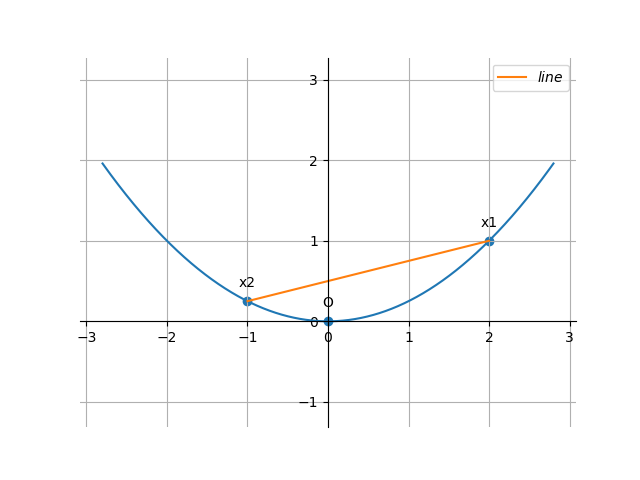
\includegraphics[width=0.75\columnwidth]{conic.png}
\caption{Tangents from A to circle through B, C and D}
\label{fig:triangle}
\end{figure}

The given equation of parabola $x^2 = 4y$ can be written in the general quadratic form as
\begin{align}
    \label{eq:conic_quad_form}
    \vec{x}^{\top}\vec{V}\vec{x}+2\vec{u}^{\top}\vec{x}+f=0
    \end{align}
where
\begin{align}
	\label{eq:V_matrix}
	\vec{V} &= \myvec{1 & 0\\0 & 0},
	\\
	\label{eq:u_vector}
	\vec{u} &= \myvec{0\\-2},
	\\
	\label{eq:f_value}
	f &= 0
	%\\
\end{align}

Let the point from which normals are drawn be $\vec{h}$. Then, the equation of the normal can be written as
\begin{align}
	\vec{x} = \vec{h} + \lambda\vec{m}
	\label{eq:normal_chord}
\end{align}
Say the point of intersection of \eqref{eq:normal_chord} with the conic is $\vec{q}$. A tangent drawn at $\vec{q}$ satisfies the equation
\begin{align}
	\label{eq:tangency_condition}
	\vec{n}^\top(\vec{Vq}+\vec{u}) = 0
\end{align}
Where $\vec{n}$ is the direction vector of the tangent and is perpendicular to $\vec{m}$ in \eqref{eq:normal_chord}.\\\\
In general, the parameter values for points of intersection of a line given by \eqref{eq:normal_chord} with a conic is given by
{\tiny
\begin{multline}
\lambda_i = \frac{1}
{
\vec{m}^T\vec{V}\vec{m}
}
\lbrak{-\vec{m}^T\brak{\vec{V}\vec{h}+\vec{u}}}
\\
\pm
\rbrak{\sqrt{
\sbrak{
\vec{m}^T\brak{\vec{V}\vec{h}+\vec{u}}
}^2
-
\brak
{
\vec{h}^T\vec{V}\vec{h} + 2\vec{u}^T\vec{h} +f
}
\brak{\vec{m}^T\vec{V}\vec{m}}
}
}
\label{eq:tangent_roots}
\end{multline}
}
Using \eqref{eq:tangent_roots} and \eqref{eq:normal_chord}, the intersection point $\vec{q}$ can be written as
\begin{align}
	\label{eq:point_of_tangency}
	\vec{q} = \vec{h} + \lambda_i\vec{m}
\end{align}
Substituting \eqref{eq:point_of_tangency} in \eqref{eq:tangency_condition},
\begin{align}
	\label{eq:normal_simp_1}
	\vec{n}^\top(\vec{V}(\vec{h}+\lambda_i\vec{m})+\vec{u}) = 0\\
	\label{eq:normal_simp_2}
	\implies \lambda_i\vec{n}^\top\vec{V}\vec{m} = -\vec{n}^\top(\vec{Vh}+\vec{u})
\end{align}
Substituting value of $\lambda_i$ from \eqref{eq:tangent_roots} in \eqref{eq:normal_simp_2}
{\tiny
\begin{multline}
	\frac{1}{\vec{m}^\top\vec{V}\vec{m}}\lbrak{-\vec{m}^\top\brak{\vec{Vh}+\vec{u}}} \\ 
	\pm \rbrak{\sqrt{\sbrak{\vec{m}^T\brak{\vec{V}\vec{h}+\vec{u}}}^2-\brak{\vec{h}^T\vec{V}\vec{h} + 2\vec{u}^T\vec{h} +f}\brak{\vec{m}^T\vec{V}\vec{m}}}}\vec{n}^\top\vec{V}\vec{m} \\
	= -\vec{n}^\top\brak{\vec{Vh}+\vec{u}}
	\label{eq:normal_simp_3}
\end{multline}
}
Rearranging the terms,
{\tiny
\begin{multline}
	\pm \sqrt{\sbrak{\vec{m}^T\brak{\vec{V}\vec{h}+\vec{u}}}^2-\brak{\vec{h}^T\vec{V}\vec{h} + 2\vec{u}^T\vec{h} +f}\brak{\vec{m}^T\vec{V}\vec{m}}} \brak{\vec{n}^\top\vec{V}\vec{m}} \\ = \brak{\vec{Vh}+\vec{u}}^\top\brak{\brak{\vec{n}^\top\vec{V}\vec{m}}\vec{m}-\brak{\vec{m}^\top\vec{V}\vec{m}}\vec{n}}
\end{multline}
}
Squaring on both sides
{\tiny
\begin{multline}
	\sbrak{\sbrak{\vec{m}^T\brak{\vec{V}\vec{h}+\vec{u}}}^2-\brak{\vec{h}^T\vec{V}\vec{h} + 2\vec{u}^T\vec{h} +f}\brak{\vec{m}^T\vec{V}\vec{m}}}\brak{\vec{n}^\top\vec{V}\vec{m}}^2 \\ = \sbrak{\brak{\vec{Vh}+\vec{u}}^\top\brak{\brak{\vec{n}^\top\vec{V}\vec{m}}\vec{m}-\brak{\vec{m}^\top\vec{V}\vec{m}}\vec{n}}}^2
	\label{eq:normal_solution}
\end{multline}
}\\
If $\vec{n}$ is taken as $\myvec{-\mu \\ 1}$, then $\vec{m}$ is $\myvec{-1 \\ -\mu}$. Substituting these values in \eqref{eq:normal_solution} and solving for $\mu$, the different possible normals passing through $\vec{h}$ are obtained.\\\\
Thus after solving we get the following values for $\mu$ = {-1, 1/2 - sqrt(3)*I/2, 1/2 + sqrt(3)*I/2}\\\\
Taking $\mu$=1 we get,
\begin{center}
$\vec{n} = \myvec{1 \\ 1}$, $\vec{m} = \myvec{-1 \\ 1}$\\
\end{center}
By calculating $\lambda_i$ from \eqref{eq:normal_simp_2}, we get
\begin{center}
    $\lambda_i = -1$
\end{center}
We find out $\vec{q}$ from \eqref{eq:point_of_tangency},
\begin{center}
where $\vec{h} = \myvec{1 \\ 2}$, $\vec{m} = \myvec{-1 \\ 1}$, $\lambda_i = -1$
\end{center}
\begin{center}
    $\vec{q} = \myvec{1 \\ 2} + (-1)\myvec{-1 \\ 1} = $\myvec{2 \\ 1}
\end{center}
\begin{center}
    Thus $\vec{q}$ satisfies Option(a) i.e. $x+y=3$
\end{center} 

\section*{\large Construction}
{
\setlength\extrarowheight{5pt}
\begin{tabular}{|c|c|c|}
	\hline
	\textbf{Symbol}&\textbf{Value}&\textbf{Description}\\[5pt]
	\hline
	$\vec{h}$&$\myvec{1 \\ 2}$&Given point through which Normal is passing\\[5pt]
	\hline
	$\vec{q}$&$\myvec{2 \\ 1}$&Foot of Normal\\[5pt]
	\hline
	$\vec{m}$ & $\myvec{-1 \\ 1}$ & Direction Vector of Normal\\[5pt]
	\hline
	$\vec{n}$ & $\myvec{1 \\ 1}$ & Direction Vector of Tangent at $\myvec{q}$\\
	\hline
\end{tabular}
}

\end{document}
\fi

\item 
Find the equation of the tangent line to the curve
\begin{align}
y=x^2-2x+7
\end{align}
\begin{enumerate}
    \item parallel to the line $2x-y+9=0$.
    \item perpendicular to the line $5y-15x=13$.
\end{enumerate}
\solution
\label{chapters/12/6/3/15}
\iffalse
\documentclass[journal,10pt,twocolumn]{article}
\usepackage{graphicx, float}
\usepackage[margin=0.5in]{geometry}
\usepackage{amsmath, bm}
\usepackage{array}
\usepackage{booktabs}
\usepackage[utf8]{inputenc}
\usepackage{amsfonts}
\usepackage{amssymb}
\usepackage{graphicx}
\usepackage{multicol}
\usepackage{tabularx}
\usepackage{hyperref}
\usepackage{mathtools}
\DeclareUnicodeCharacter{2212}{-}
\providecommand{\norm}[1]{\left\lVert#1\right\rVert}
\providecommand{\abs}[1]{\left\vert#1\right\vert}
\let\vec\mathbf
\newcommand{\myvec}[1]{\ensuremath{\begin{pmatrix}#1\end{pmatrix}}}
\newcommand{\mydet}[1]{\ensuremath{\begin{vmatrix}#1\end{vmatrix}}}
\providecommand{\brak}[1]{\ensuremath{\left(#1\right)}}
\providecommand{\lbrak}[1]{\ensuremath{\left(#1\right.}}
\providecommand{\rbrak}[1]{\ensuremath{\left.#1\right)}}
\providecommand{\sbrak}[1]{\ensuremath{{}\left[#1\right]}}
%\providecommand{\norm}[1]{\left\lVert#1\right\rVert}
%\providecommand{\sbrak}[1]{\ensuremath{{}\left[#1\right]}}
%\providecommand{\lsbrak}[1]{\ensuremath{{}\left[#1\right.}}
%\providecommand{\rsbrak}[1]{\ensuremath{{}\left.#1\right]}}
%\providecommand{\brak}[1]{\ensuremath{\left(#1\right)}}
%\providecommand{\lbrak}[1]{\ensuremath{\left(#1\right.}}
%\providecommand{\rbrak}[1]{\ensuremath{\left.#1\right)}}
%\providecommand{\cbrak}[1]{\ensuremath{\left\{#1\right\}}}
%\providecommand{\lcbrak}[1]{\ensuremath{\left\{#1\right.}}
%\providecommand{\rcbrak}[1]{\ensuremath{\left.#1\right\}}}
%\newcommand{\myvec}[1]{\ensuremath{\begin{pmatrix}#1\end{pmatrix}}}
%\let\vec\mathbf

\title{\textbf{Conic Assignment}}
\author{Namrath Pinnamaneni \hspace{9cm} FWC22042}
\date{September 2022}

\begin{document}

\maketitle
\paragraph{\textit{Problem Statement} -
\fi
Find the normal to the curve $x_2=4y$ passing (1,2). 
\iffalse
(a)x+y=3  \hspace{2cm} (b)x-y=3\\ 
(c)x+y=1 \hspace{2cm}  (d)x-y=1\\}

\section*{\large Solution}

\begin{figure}[H]
\centering
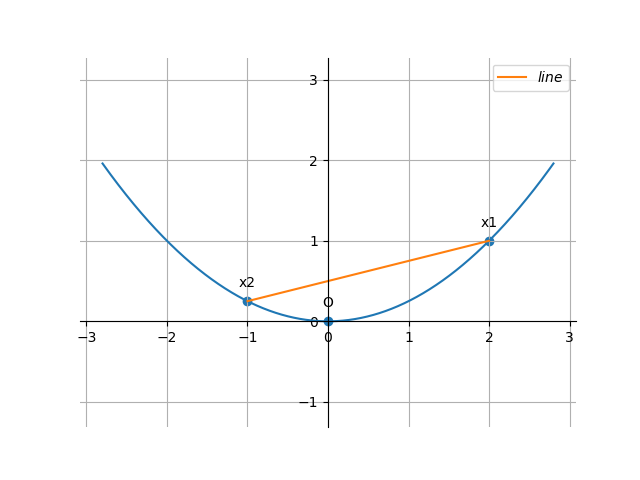
\includegraphics[width=0.75\columnwidth]{conic.png}
\caption{Tangents from A to circle through B, C and D}
\label{fig:triangle}
\end{figure}

The given equation of parabola $x^2 = 4y$ can be written in the general quadratic form as
\begin{align}
    \label{eq:conic_quad_form}
    \vec{x}^{\top}\vec{V}\vec{x}+2\vec{u}^{\top}\vec{x}+f=0
    \end{align}
where
\begin{align}
	\label{eq:V_matrix}
	\vec{V} &= \myvec{1 & 0\\0 & 0},
	\\
	\label{eq:u_vector}
	\vec{u} &= \myvec{0\\-2},
	\\
	\label{eq:f_value}
	f &= 0
	%\\
\end{align}

Let the point from which normals are drawn be $\vec{h}$. Then, the equation of the normal can be written as
\begin{align}
	\vec{x} = \vec{h} + \lambda\vec{m}
	\label{eq:normal_chord}
\end{align}
Say the point of intersection of \eqref{eq:normal_chord} with the conic is $\vec{q}$. A tangent drawn at $\vec{q}$ satisfies the equation
\begin{align}
	\label{eq:tangency_condition}
	\vec{n}^\top(\vec{Vq}+\vec{u}) = 0
\end{align}
Where $\vec{n}$ is the direction vector of the tangent and is perpendicular to $\vec{m}$ in \eqref{eq:normal_chord}.\\\\
In general, the parameter values for points of intersection of a line given by \eqref{eq:normal_chord} with a conic is given by
{\tiny
\begin{multline}
\lambda_i = \frac{1}
{
\vec{m}^T\vec{V}\vec{m}
}
\lbrak{-\vec{m}^T\brak{\vec{V}\vec{h}+\vec{u}}}
\\
\pm
\rbrak{\sqrt{
\sbrak{
\vec{m}^T\brak{\vec{V}\vec{h}+\vec{u}}
}^2
-
\brak
{
\vec{h}^T\vec{V}\vec{h} + 2\vec{u}^T\vec{h} +f
}
\brak{\vec{m}^T\vec{V}\vec{m}}
}
}
\label{eq:tangent_roots}
\end{multline}
}
Using \eqref{eq:tangent_roots} and \eqref{eq:normal_chord}, the intersection point $\vec{q}$ can be written as
\begin{align}
	\label{eq:point_of_tangency}
	\vec{q} = \vec{h} + \lambda_i\vec{m}
\end{align}
Substituting \eqref{eq:point_of_tangency} in \eqref{eq:tangency_condition},
\begin{align}
	\label{eq:normal_simp_1}
	\vec{n}^\top(\vec{V}(\vec{h}+\lambda_i\vec{m})+\vec{u}) = 0\\
	\label{eq:normal_simp_2}
	\implies \lambda_i\vec{n}^\top\vec{V}\vec{m} = -\vec{n}^\top(\vec{Vh}+\vec{u})
\end{align}
Substituting value of $\lambda_i$ from \eqref{eq:tangent_roots} in \eqref{eq:normal_simp_2}
{\tiny
\begin{multline}
	\frac{1}{\vec{m}^\top\vec{V}\vec{m}}\lbrak{-\vec{m}^\top\brak{\vec{Vh}+\vec{u}}} \\ 
	\pm \rbrak{\sqrt{\sbrak{\vec{m}^T\brak{\vec{V}\vec{h}+\vec{u}}}^2-\brak{\vec{h}^T\vec{V}\vec{h} + 2\vec{u}^T\vec{h} +f}\brak{\vec{m}^T\vec{V}\vec{m}}}}\vec{n}^\top\vec{V}\vec{m} \\
	= -\vec{n}^\top\brak{\vec{Vh}+\vec{u}}
	\label{eq:normal_simp_3}
\end{multline}
}
Rearranging the terms,
{\tiny
\begin{multline}
	\pm \sqrt{\sbrak{\vec{m}^T\brak{\vec{V}\vec{h}+\vec{u}}}^2-\brak{\vec{h}^T\vec{V}\vec{h} + 2\vec{u}^T\vec{h} +f}\brak{\vec{m}^T\vec{V}\vec{m}}} \brak{\vec{n}^\top\vec{V}\vec{m}} \\ = \brak{\vec{Vh}+\vec{u}}^\top\brak{\brak{\vec{n}^\top\vec{V}\vec{m}}\vec{m}-\brak{\vec{m}^\top\vec{V}\vec{m}}\vec{n}}
\end{multline}
}
Squaring on both sides
{\tiny
\begin{multline}
	\sbrak{\sbrak{\vec{m}^T\brak{\vec{V}\vec{h}+\vec{u}}}^2-\brak{\vec{h}^T\vec{V}\vec{h} + 2\vec{u}^T\vec{h} +f}\brak{\vec{m}^T\vec{V}\vec{m}}}\brak{\vec{n}^\top\vec{V}\vec{m}}^2 \\ = \sbrak{\brak{\vec{Vh}+\vec{u}}^\top\brak{\brak{\vec{n}^\top\vec{V}\vec{m}}\vec{m}-\brak{\vec{m}^\top\vec{V}\vec{m}}\vec{n}}}^2
	\label{eq:normal_solution}
\end{multline}
}\\
If $\vec{n}$ is taken as $\myvec{-\mu \\ 1}$, then $\vec{m}$ is $\myvec{-1 \\ -\mu}$. Substituting these values in \eqref{eq:normal_solution} and solving for $\mu$, the different possible normals passing through $\vec{h}$ are obtained.\\\\
Thus after solving we get the following values for $\mu$ = {-1, 1/2 - sqrt(3)*I/2, 1/2 + sqrt(3)*I/2}\\\\
Taking $\mu$=1 we get,
\begin{center}
$\vec{n} = \myvec{1 \\ 1}$, $\vec{m} = \myvec{-1 \\ 1}$\\
\end{center}
By calculating $\lambda_i$ from \eqref{eq:normal_simp_2}, we get
\begin{center}
    $\lambda_i = -1$
\end{center}
We find out $\vec{q}$ from \eqref{eq:point_of_tangency},
\begin{center}
where $\vec{h} = \myvec{1 \\ 2}$, $\vec{m} = \myvec{-1 \\ 1}$, $\lambda_i = -1$
\end{center}
\begin{center}
    $\vec{q} = \myvec{1 \\ 2} + (-1)\myvec{-1 \\ 1} = $\myvec{2 \\ 1}
\end{center}
\begin{center}
    Thus $\vec{q}$ satisfies Option(a) i.e. $x+y=3$
\end{center} 

\section*{\large Construction}
{
\setlength\extrarowheight{5pt}
\begin{tabular}{|c|c|c|}
	\hline
	\textbf{Symbol}&\textbf{Value}&\textbf{Description}\\[5pt]
	\hline
	$\vec{h}$&$\myvec{1 \\ 2}$&Given point through which Normal is passing\\[5pt]
	\hline
	$\vec{q}$&$\myvec{2 \\ 1}$&Foot of Normal\\[5pt]
	\hline
	$\vec{m}$ & $\myvec{-1 \\ 1}$ & Direction Vector of Normal\\[5pt]
	\hline
	$\vec{n}$ & $\myvec{1 \\ 1}$ & Direction Vector of Tangent at $\myvec{q}$\\
	\hline
\end{tabular}
}

\end{document}
\fi

\item 
Find the equation of the tangent to the curve 
\begin{align}
	y = \sqrt{3x-2}
\end{align}
which is parallel to the line
\begin{align}
	4x-2y+5 = 0
\end{align}
\solution 
\label{chapters/12/6/3/25}
\iffalse
\documentclass[journal,10pt,twocolumn]{article}
\usepackage{graphicx, float}
\usepackage[margin=0.5in]{geometry}
\usepackage{amsmath, bm}
\usepackage{array}
\usepackage{booktabs}
\usepackage[utf8]{inputenc}
\usepackage{amsfonts}
\usepackage{amssymb}
\usepackage{graphicx}
\usepackage{multicol}
\usepackage{tabularx}
\usepackage{hyperref}
\usepackage{mathtools}
\DeclareUnicodeCharacter{2212}{-}
\providecommand{\norm}[1]{\left\lVert#1\right\rVert}
\providecommand{\abs}[1]{\left\vert#1\right\vert}
\let\vec\mathbf
\newcommand{\myvec}[1]{\ensuremath{\begin{pmatrix}#1\end{pmatrix}}}
\newcommand{\mydet}[1]{\ensuremath{\begin{vmatrix}#1\end{vmatrix}}}
\providecommand{\brak}[1]{\ensuremath{\left(#1\right)}}
\providecommand{\lbrak}[1]{\ensuremath{\left(#1\right.}}
\providecommand{\rbrak}[1]{\ensuremath{\left.#1\right)}}
\providecommand{\sbrak}[1]{\ensuremath{{}\left[#1\right]}}
%\providecommand{\norm}[1]{\left\lVert#1\right\rVert}
%\providecommand{\sbrak}[1]{\ensuremath{{}\left[#1\right]}}
%\providecommand{\lsbrak}[1]{\ensuremath{{}\left[#1\right.}}
%\providecommand{\rsbrak}[1]{\ensuremath{{}\left.#1\right]}}
%\providecommand{\brak}[1]{\ensuremath{\left(#1\right)}}
%\providecommand{\lbrak}[1]{\ensuremath{\left(#1\right.}}
%\providecommand{\rbrak}[1]{\ensuremath{\left.#1\right)}}
%\providecommand{\cbrak}[1]{\ensuremath{\left\{#1\right\}}}
%\providecommand{\lcbrak}[1]{\ensuremath{\left\{#1\right.}}
%\providecommand{\rcbrak}[1]{\ensuremath{\left.#1\right\}}}
%\newcommand{\myvec}[1]{\ensuremath{\begin{pmatrix}#1\end{pmatrix}}}
%\let\vec\mathbf

\title{\textbf{Conic Assignment}}
\author{Namrath Pinnamaneni \hspace{9cm} FWC22042}
\date{September 2022}

\begin{document}

\maketitle
\paragraph{\textit{Problem Statement} -
\fi
Find the normal to the curve $x_2=4y$ passing (1,2). 
\iffalse
(a)x+y=3  \hspace{2cm} (b)x-y=3\\ 
(c)x+y=1 \hspace{2cm}  (d)x-y=1\\}

\section*{\large Solution}

\begin{figure}[H]
\centering
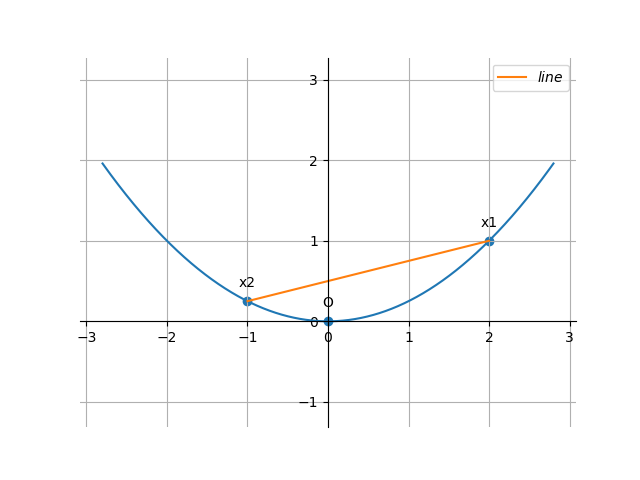
\includegraphics[width=0.75\columnwidth]{conic.png}
\caption{Tangents from A to circle through B, C and D}
\label{fig:triangle}
\end{figure}

The given equation of parabola $x^2 = 4y$ can be written in the general quadratic form as
\begin{align}
    \label{eq:conic_quad_form}
    \vec{x}^{\top}\vec{V}\vec{x}+2\vec{u}^{\top}\vec{x}+f=0
    \end{align}
where
\begin{align}
	\label{eq:V_matrix}
	\vec{V} &= \myvec{1 & 0\\0 & 0},
	\\
	\label{eq:u_vector}
	\vec{u} &= \myvec{0\\-2},
	\\
	\label{eq:f_value}
	f &= 0
	%\\
\end{align}

Let the point from which normals are drawn be $\vec{h}$. Then, the equation of the normal can be written as
\begin{align}
	\vec{x} = \vec{h} + \lambda\vec{m}
	\label{eq:normal_chord}
\end{align}
Say the point of intersection of \eqref{eq:normal_chord} with the conic is $\vec{q}$. A tangent drawn at $\vec{q}$ satisfies the equation
\begin{align}
	\label{eq:tangency_condition}
	\vec{n}^\top(\vec{Vq}+\vec{u}) = 0
\end{align}
Where $\vec{n}$ is the direction vector of the tangent and is perpendicular to $\vec{m}$ in \eqref{eq:normal_chord}.\\\\
In general, the parameter values for points of intersection of a line given by \eqref{eq:normal_chord} with a conic is given by
{\tiny
\begin{multline}
\lambda_i = \frac{1}
{
\vec{m}^T\vec{V}\vec{m}
}
\lbrak{-\vec{m}^T\brak{\vec{V}\vec{h}+\vec{u}}}
\\
\pm
\rbrak{\sqrt{
\sbrak{
\vec{m}^T\brak{\vec{V}\vec{h}+\vec{u}}
}^2
-
\brak
{
\vec{h}^T\vec{V}\vec{h} + 2\vec{u}^T\vec{h} +f
}
\brak{\vec{m}^T\vec{V}\vec{m}}
}
}
\label{eq:tangent_roots}
\end{multline}
}
Using \eqref{eq:tangent_roots} and \eqref{eq:normal_chord}, the intersection point $\vec{q}$ can be written as
\begin{align}
	\label{eq:point_of_tangency}
	\vec{q} = \vec{h} + \lambda_i\vec{m}
\end{align}
Substituting \eqref{eq:point_of_tangency} in \eqref{eq:tangency_condition},
\begin{align}
	\label{eq:normal_simp_1}
	\vec{n}^\top(\vec{V}(\vec{h}+\lambda_i\vec{m})+\vec{u}) = 0\\
	\label{eq:normal_simp_2}
	\implies \lambda_i\vec{n}^\top\vec{V}\vec{m} = -\vec{n}^\top(\vec{Vh}+\vec{u})
\end{align}
Substituting value of $\lambda_i$ from \eqref{eq:tangent_roots} in \eqref{eq:normal_simp_2}
{\tiny
\begin{multline}
	\frac{1}{\vec{m}^\top\vec{V}\vec{m}}\lbrak{-\vec{m}^\top\brak{\vec{Vh}+\vec{u}}} \\ 
	\pm \rbrak{\sqrt{\sbrak{\vec{m}^T\brak{\vec{V}\vec{h}+\vec{u}}}^2-\brak{\vec{h}^T\vec{V}\vec{h} + 2\vec{u}^T\vec{h} +f}\brak{\vec{m}^T\vec{V}\vec{m}}}}\vec{n}^\top\vec{V}\vec{m} \\
	= -\vec{n}^\top\brak{\vec{Vh}+\vec{u}}
	\label{eq:normal_simp_3}
\end{multline}
}
Rearranging the terms,
{\tiny
\begin{multline}
	\pm \sqrt{\sbrak{\vec{m}^T\brak{\vec{V}\vec{h}+\vec{u}}}^2-\brak{\vec{h}^T\vec{V}\vec{h} + 2\vec{u}^T\vec{h} +f}\brak{\vec{m}^T\vec{V}\vec{m}}} \brak{\vec{n}^\top\vec{V}\vec{m}} \\ = \brak{\vec{Vh}+\vec{u}}^\top\brak{\brak{\vec{n}^\top\vec{V}\vec{m}}\vec{m}-\brak{\vec{m}^\top\vec{V}\vec{m}}\vec{n}}
\end{multline}
}
Squaring on both sides
{\tiny
\begin{multline}
	\sbrak{\sbrak{\vec{m}^T\brak{\vec{V}\vec{h}+\vec{u}}}^2-\brak{\vec{h}^T\vec{V}\vec{h} + 2\vec{u}^T\vec{h} +f}\brak{\vec{m}^T\vec{V}\vec{m}}}\brak{\vec{n}^\top\vec{V}\vec{m}}^2 \\ = \sbrak{\brak{\vec{Vh}+\vec{u}}^\top\brak{\brak{\vec{n}^\top\vec{V}\vec{m}}\vec{m}-\brak{\vec{m}^\top\vec{V}\vec{m}}\vec{n}}}^2
	\label{eq:normal_solution}
\end{multline}
}\\
If $\vec{n}$ is taken as $\myvec{-\mu \\ 1}$, then $\vec{m}$ is $\myvec{-1 \\ -\mu}$. Substituting these values in \eqref{eq:normal_solution} and solving for $\mu$, the different possible normals passing through $\vec{h}$ are obtained.\\\\
Thus after solving we get the following values for $\mu$ = {-1, 1/2 - sqrt(3)*I/2, 1/2 + sqrt(3)*I/2}\\\\
Taking $\mu$=1 we get,
\begin{center}
$\vec{n} = \myvec{1 \\ 1}$, $\vec{m} = \myvec{-1 \\ 1}$\\
\end{center}
By calculating $\lambda_i$ from \eqref{eq:normal_simp_2}, we get
\begin{center}
    $\lambda_i = -1$
\end{center}
We find out $\vec{q}$ from \eqref{eq:point_of_tangency},
\begin{center}
where $\vec{h} = \myvec{1 \\ 2}$, $\vec{m} = \myvec{-1 \\ 1}$, $\lambda_i = -1$
\end{center}
\begin{center}
    $\vec{q} = \myvec{1 \\ 2} + (-1)\myvec{-1 \\ 1} = $\myvec{2 \\ 1}
\end{center}
\begin{center}
    Thus $\vec{q}$ satisfies Option(a) i.e. $x+y=3$
\end{center} 

\section*{\large Construction}
{
\setlength\extrarowheight{5pt}
\begin{tabular}{|c|c|c|}
	\hline
	\textbf{Symbol}&\textbf{Value}&\textbf{Description}\\[5pt]
	\hline
	$\vec{h}$&$\myvec{1 \\ 2}$&Given point through which Normal is passing\\[5pt]
	\hline
	$\vec{q}$&$\myvec{2 \\ 1}$&Foot of Normal\\[5pt]
	\hline
	$\vec{m}$ & $\myvec{-1 \\ 1}$ & Direction Vector of Normal\\[5pt]
	\hline
	$\vec{n}$ & $\myvec{1 \\ 1}$ & Direction Vector of Tangent at $\myvec{q}$\\
	\hline
\end{tabular}
}

\end{document}
\fi

\item 
Find the point at which the line $y = x + 1$ is a tangent to the curve $y^2 = 4x$.
\\
\solution 
\label{chapters/12/6/3/27}
\iffalse
\documentclass[journal,10pt,twocolumn]{article}
\usepackage{graphicx, float}
\usepackage[margin=0.5in]{geometry}
\usepackage{amsmath, bm}
\usepackage{array}
\usepackage{booktabs}
\usepackage[utf8]{inputenc}
\usepackage{amsfonts}
\usepackage{amssymb}
\usepackage{graphicx}
\usepackage{multicol}
\usepackage{tabularx}
\usepackage{hyperref}
\usepackage{mathtools}
\DeclareUnicodeCharacter{2212}{-}
\providecommand{\norm}[1]{\left\lVert#1\right\rVert}
\providecommand{\abs}[1]{\left\vert#1\right\vert}
\let\vec\mathbf
\newcommand{\myvec}[1]{\ensuremath{\begin{pmatrix}#1\end{pmatrix}}}
\newcommand{\mydet}[1]{\ensuremath{\begin{vmatrix}#1\end{vmatrix}}}
\providecommand{\brak}[1]{\ensuremath{\left(#1\right)}}
\providecommand{\lbrak}[1]{\ensuremath{\left(#1\right.}}
\providecommand{\rbrak}[1]{\ensuremath{\left.#1\right)}}
\providecommand{\sbrak}[1]{\ensuremath{{}\left[#1\right]}}
%\providecommand{\norm}[1]{\left\lVert#1\right\rVert}
%\providecommand{\sbrak}[1]{\ensuremath{{}\left[#1\right]}}
%\providecommand{\lsbrak}[1]{\ensuremath{{}\left[#1\right.}}
%\providecommand{\rsbrak}[1]{\ensuremath{{}\left.#1\right]}}
%\providecommand{\brak}[1]{\ensuremath{\left(#1\right)}}
%\providecommand{\lbrak}[1]{\ensuremath{\left(#1\right.}}
%\providecommand{\rbrak}[1]{\ensuremath{\left.#1\right)}}
%\providecommand{\cbrak}[1]{\ensuremath{\left\{#1\right\}}}
%\providecommand{\lcbrak}[1]{\ensuremath{\left\{#1\right.}}
%\providecommand{\rcbrak}[1]{\ensuremath{\left.#1\right\}}}
%\newcommand{\myvec}[1]{\ensuremath{\begin{pmatrix}#1\end{pmatrix}}}
%\let\vec\mathbf

\title{\textbf{Conic Assignment}}
\author{Namrath Pinnamaneni \hspace{9cm} FWC22042}
\date{September 2022}

\begin{document}

\maketitle
\paragraph{\textit{Problem Statement} -
\fi
Find the normal to the curve $x_2=4y$ passing (1,2). 
\iffalse
(a)x+y=3  \hspace{2cm} (b)x-y=3\\ 
(c)x+y=1 \hspace{2cm}  (d)x-y=1\\}

\section*{\large Solution}

\begin{figure}[H]
\centering
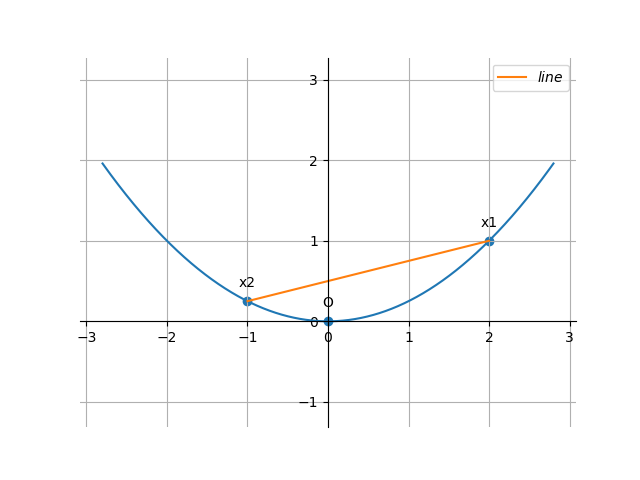
\includegraphics[width=0.75\columnwidth]{conic.png}
\caption{Tangents from A to circle through B, C and D}
\label{fig:triangle}
\end{figure}

The given equation of parabola $x^2 = 4y$ can be written in the general quadratic form as
\begin{align}
    \label{eq:conic_quad_form}
    \vec{x}^{\top}\vec{V}\vec{x}+2\vec{u}^{\top}\vec{x}+f=0
    \end{align}
where
\begin{align}
	\label{eq:V_matrix}
	\vec{V} &= \myvec{1 & 0\\0 & 0},
	\\
	\label{eq:u_vector}
	\vec{u} &= \myvec{0\\-2},
	\\
	\label{eq:f_value}
	f &= 0
	%\\
\end{align}

Let the point from which normals are drawn be $\vec{h}$. Then, the equation of the normal can be written as
\begin{align}
	\vec{x} = \vec{h} + \lambda\vec{m}
	\label{eq:normal_chord}
\end{align}
Say the point of intersection of \eqref{eq:normal_chord} with the conic is $\vec{q}$. A tangent drawn at $\vec{q}$ satisfies the equation
\begin{align}
	\label{eq:tangency_condition}
	\vec{n}^\top(\vec{Vq}+\vec{u}) = 0
\end{align}
Where $\vec{n}$ is the direction vector of the tangent and is perpendicular to $\vec{m}$ in \eqref{eq:normal_chord}.\\\\
In general, the parameter values for points of intersection of a line given by \eqref{eq:normal_chord} with a conic is given by
{\tiny
\begin{multline}
\lambda_i = \frac{1}
{
\vec{m}^T\vec{V}\vec{m}
}
\lbrak{-\vec{m}^T\brak{\vec{V}\vec{h}+\vec{u}}}
\\
\pm
\rbrak{\sqrt{
\sbrak{
\vec{m}^T\brak{\vec{V}\vec{h}+\vec{u}}
}^2
-
\brak
{
\vec{h}^T\vec{V}\vec{h} + 2\vec{u}^T\vec{h} +f
}
\brak{\vec{m}^T\vec{V}\vec{m}}
}
}
\label{eq:tangent_roots}
\end{multline}
}
Using \eqref{eq:tangent_roots} and \eqref{eq:normal_chord}, the intersection point $\vec{q}$ can be written as
\begin{align}
	\label{eq:point_of_tangency}
	\vec{q} = \vec{h} + \lambda_i\vec{m}
\end{align}
Substituting \eqref{eq:point_of_tangency} in \eqref{eq:tangency_condition},
\begin{align}
	\label{eq:normal_simp_1}
	\vec{n}^\top(\vec{V}(\vec{h}+\lambda_i\vec{m})+\vec{u}) = 0\\
	\label{eq:normal_simp_2}
	\implies \lambda_i\vec{n}^\top\vec{V}\vec{m} = -\vec{n}^\top(\vec{Vh}+\vec{u})
\end{align}
Substituting value of $\lambda_i$ from \eqref{eq:tangent_roots} in \eqref{eq:normal_simp_2}
{\tiny
\begin{multline}
	\frac{1}{\vec{m}^\top\vec{V}\vec{m}}\lbrak{-\vec{m}^\top\brak{\vec{Vh}+\vec{u}}} \\ 
	\pm \rbrak{\sqrt{\sbrak{\vec{m}^T\brak{\vec{V}\vec{h}+\vec{u}}}^2-\brak{\vec{h}^T\vec{V}\vec{h} + 2\vec{u}^T\vec{h} +f}\brak{\vec{m}^T\vec{V}\vec{m}}}}\vec{n}^\top\vec{V}\vec{m} \\
	= -\vec{n}^\top\brak{\vec{Vh}+\vec{u}}
	\label{eq:normal_simp_3}
\end{multline}
}
Rearranging the terms,
{\tiny
\begin{multline}
	\pm \sqrt{\sbrak{\vec{m}^T\brak{\vec{V}\vec{h}+\vec{u}}}^2-\brak{\vec{h}^T\vec{V}\vec{h} + 2\vec{u}^T\vec{h} +f}\brak{\vec{m}^T\vec{V}\vec{m}}} \brak{\vec{n}^\top\vec{V}\vec{m}} \\ = \brak{\vec{Vh}+\vec{u}}^\top\brak{\brak{\vec{n}^\top\vec{V}\vec{m}}\vec{m}-\brak{\vec{m}^\top\vec{V}\vec{m}}\vec{n}}
\end{multline}
}
Squaring on both sides
{\tiny
\begin{multline}
	\sbrak{\sbrak{\vec{m}^T\brak{\vec{V}\vec{h}+\vec{u}}}^2-\brak{\vec{h}^T\vec{V}\vec{h} + 2\vec{u}^T\vec{h} +f}\brak{\vec{m}^T\vec{V}\vec{m}}}\brak{\vec{n}^\top\vec{V}\vec{m}}^2 \\ = \sbrak{\brak{\vec{Vh}+\vec{u}}^\top\brak{\brak{\vec{n}^\top\vec{V}\vec{m}}\vec{m}-\brak{\vec{m}^\top\vec{V}\vec{m}}\vec{n}}}^2
	\label{eq:normal_solution}
\end{multline}
}\\
If $\vec{n}$ is taken as $\myvec{-\mu \\ 1}$, then $\vec{m}$ is $\myvec{-1 \\ -\mu}$. Substituting these values in \eqref{eq:normal_solution} and solving for $\mu$, the different possible normals passing through $\vec{h}$ are obtained.\\\\
Thus after solving we get the following values for $\mu$ = {-1, 1/2 - sqrt(3)*I/2, 1/2 + sqrt(3)*I/2}\\\\
Taking $\mu$=1 we get,
\begin{center}
$\vec{n} = \myvec{1 \\ 1}$, $\vec{m} = \myvec{-1 \\ 1}$\\
\end{center}
By calculating $\lambda_i$ from \eqref{eq:normal_simp_2}, we get
\begin{center}
    $\lambda_i = -1$
\end{center}
We find out $\vec{q}$ from \eqref{eq:point_of_tangency},
\begin{center}
where $\vec{h} = \myvec{1 \\ 2}$, $\vec{m} = \myvec{-1 \\ 1}$, $\lambda_i = -1$
\end{center}
\begin{center}
    $\vec{q} = \myvec{1 \\ 2} + (-1)\myvec{-1 \\ 1} = $\myvec{2 \\ 1}
\end{center}
\begin{center}
    Thus $\vec{q}$ satisfies Option(a) i.e. $x+y=3$
\end{center} 

\section*{\large Construction}
{
\setlength\extrarowheight{5pt}
\begin{tabular}{|c|c|c|}
	\hline
	\textbf{Symbol}&\textbf{Value}&\textbf{Description}\\[5pt]
	\hline
	$\vec{h}$&$\myvec{1 \\ 2}$&Given point through which Normal is passing\\[5pt]
	\hline
	$\vec{q}$&$\myvec{2 \\ 1}$&Foot of Normal\\[5pt]
	\hline
	$\vec{m}$ & $\myvec{-1 \\ 1}$ & Direction Vector of Normal\\[5pt]
	\hline
	$\vec{n}$ & $\myvec{1 \\ 1}$ & Direction Vector of Tangent at $\myvec{q}$\\
	\hline
\end{tabular}
}

\end{document}
\fi

    \item The point on the curve 
\label{chapters/12/6/5/27}
    \begin{align}
        x^2 = 2y
        \label{eq:chapters/12/6/5/27/curve}
    \end{align}
    which is nearest to the point 
    $\vec{P} = \myvec{0\\5}$ is
    \begin{enumerate}
        \item $\myvec{2\sqrt{2}\\4}$
        \item $\myvec{2\sqrt{2}\\0}$
        \item $\myvec{0\\0}$
        \item $\myvec{2\\2}$
    \end{enumerate}
    \solution 
\iffalse
\documentclass[journal,10pt,twocolumn]{article}
\usepackage{graphicx, float}
\usepackage[margin=0.5in]{geometry}
\usepackage{amsmath, bm}
\usepackage{array}
\usepackage{booktabs}
\usepackage[utf8]{inputenc}
\usepackage{amsfonts}
\usepackage{amssymb}
\usepackage{graphicx}
\usepackage{multicol}
\usepackage{tabularx}
\usepackage{hyperref}
\usepackage{mathtools}
\DeclareUnicodeCharacter{2212}{-}
\providecommand{\norm}[1]{\left\lVert#1\right\rVert}
\providecommand{\abs}[1]{\left\vert#1\right\vert}
\let\vec\mathbf
\newcommand{\myvec}[1]{\ensuremath{\begin{pmatrix}#1\end{pmatrix}}}
\newcommand{\mydet}[1]{\ensuremath{\begin{vmatrix}#1\end{vmatrix}}}
\providecommand{\brak}[1]{\ensuremath{\left(#1\right)}}
\providecommand{\lbrak}[1]{\ensuremath{\left(#1\right.}}
\providecommand{\rbrak}[1]{\ensuremath{\left.#1\right)}}
\providecommand{\sbrak}[1]{\ensuremath{{}\left[#1\right]}}
%\providecommand{\norm}[1]{\left\lVert#1\right\rVert}
%\providecommand{\sbrak}[1]{\ensuremath{{}\left[#1\right]}}
%\providecommand{\lsbrak}[1]{\ensuremath{{}\left[#1\right.}}
%\providecommand{\rsbrak}[1]{\ensuremath{{}\left.#1\right]}}
%\providecommand{\brak}[1]{\ensuremath{\left(#1\right)}}
%\providecommand{\lbrak}[1]{\ensuremath{\left(#1\right.}}
%\providecommand{\rbrak}[1]{\ensuremath{\left.#1\right)}}
%\providecommand{\cbrak}[1]{\ensuremath{\left\{#1\right\}}}
%\providecommand{\lcbrak}[1]{\ensuremath{\left\{#1\right.}}
%\providecommand{\rcbrak}[1]{\ensuremath{\left.#1\right\}}}
%\newcommand{\myvec}[1]{\ensuremath{\begin{pmatrix}#1\end{pmatrix}}}
%\let\vec\mathbf

\title{\textbf{Conic Assignment}}
\author{Namrath Pinnamaneni \hspace{9cm} FWC22042}
\date{September 2022}

\begin{document}

\maketitle
\paragraph{\textit{Problem Statement} -
\fi
Find the normal to the curve $x_2=4y$ passing (1,2). 
\iffalse
(a)x+y=3  \hspace{2cm} (b)x-y=3\\ 
(c)x+y=1 \hspace{2cm}  (d)x-y=1\\}

\section*{\large Solution}

\begin{figure}[H]
\centering
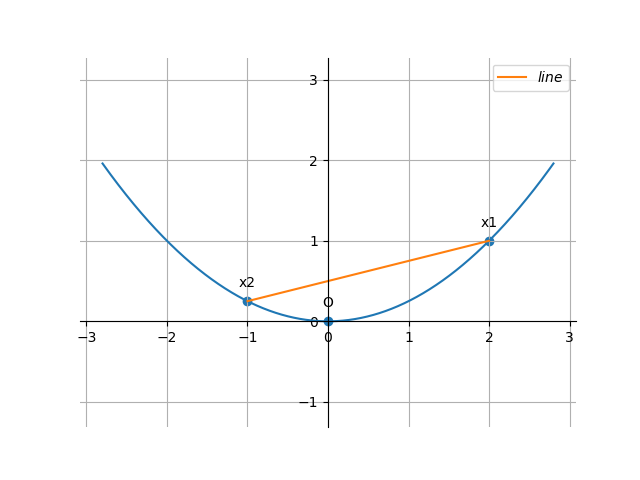
\includegraphics[width=0.75\columnwidth]{conic.png}
\caption{Tangents from A to circle through B, C and D}
\label{fig:triangle}
\end{figure}

The given equation of parabola $x^2 = 4y$ can be written in the general quadratic form as
\begin{align}
    \label{eq:conic_quad_form}
    \vec{x}^{\top}\vec{V}\vec{x}+2\vec{u}^{\top}\vec{x}+f=0
    \end{align}
where
\begin{align}
	\label{eq:V_matrix}
	\vec{V} &= \myvec{1 & 0\\0 & 0},
	\\
	\label{eq:u_vector}
	\vec{u} &= \myvec{0\\-2},
	\\
	\label{eq:f_value}
	f &= 0
	%\\
\end{align}

Let the point from which normals are drawn be $\vec{h}$. Then, the equation of the normal can be written as
\begin{align}
	\vec{x} = \vec{h} + \lambda\vec{m}
	\label{eq:normal_chord}
\end{align}
Say the point of intersection of \eqref{eq:normal_chord} with the conic is $\vec{q}$. A tangent drawn at $\vec{q}$ satisfies the equation
\begin{align}
	\label{eq:tangency_condition}
	\vec{n}^\top(\vec{Vq}+\vec{u}) = 0
\end{align}
Where $\vec{n}$ is the direction vector of the tangent and is perpendicular to $\vec{m}$ in \eqref{eq:normal_chord}.\\\\
In general, the parameter values for points of intersection of a line given by \eqref{eq:normal_chord} with a conic is given by
{\tiny
\begin{multline}
\lambda_i = \frac{1}
{
\vec{m}^T\vec{V}\vec{m}
}
\lbrak{-\vec{m}^T\brak{\vec{V}\vec{h}+\vec{u}}}
\\
\pm
\rbrak{\sqrt{
\sbrak{
\vec{m}^T\brak{\vec{V}\vec{h}+\vec{u}}
}^2
-
\brak
{
\vec{h}^T\vec{V}\vec{h} + 2\vec{u}^T\vec{h} +f
}
\brak{\vec{m}^T\vec{V}\vec{m}}
}
}
\label{eq:tangent_roots}
\end{multline}
}
Using \eqref{eq:tangent_roots} and \eqref{eq:normal_chord}, the intersection point $\vec{q}$ can be written as
\begin{align}
	\label{eq:point_of_tangency}
	\vec{q} = \vec{h} + \lambda_i\vec{m}
\end{align}
Substituting \eqref{eq:point_of_tangency} in \eqref{eq:tangency_condition},
\begin{align}
	\label{eq:normal_simp_1}
	\vec{n}^\top(\vec{V}(\vec{h}+\lambda_i\vec{m})+\vec{u}) = 0\\
	\label{eq:normal_simp_2}
	\implies \lambda_i\vec{n}^\top\vec{V}\vec{m} = -\vec{n}^\top(\vec{Vh}+\vec{u})
\end{align}
Substituting value of $\lambda_i$ from \eqref{eq:tangent_roots} in \eqref{eq:normal_simp_2}
{\tiny
\begin{multline}
	\frac{1}{\vec{m}^\top\vec{V}\vec{m}}\lbrak{-\vec{m}^\top\brak{\vec{Vh}+\vec{u}}} \\ 
	\pm \rbrak{\sqrt{\sbrak{\vec{m}^T\brak{\vec{V}\vec{h}+\vec{u}}}^2-\brak{\vec{h}^T\vec{V}\vec{h} + 2\vec{u}^T\vec{h} +f}\brak{\vec{m}^T\vec{V}\vec{m}}}}\vec{n}^\top\vec{V}\vec{m} \\
	= -\vec{n}^\top\brak{\vec{Vh}+\vec{u}}
	\label{eq:normal_simp_3}
\end{multline}
}
Rearranging the terms,
{\tiny
\begin{multline}
	\pm \sqrt{\sbrak{\vec{m}^T\brak{\vec{V}\vec{h}+\vec{u}}}^2-\brak{\vec{h}^T\vec{V}\vec{h} + 2\vec{u}^T\vec{h} +f}\brak{\vec{m}^T\vec{V}\vec{m}}} \brak{\vec{n}^\top\vec{V}\vec{m}} \\ = \brak{\vec{Vh}+\vec{u}}^\top\brak{\brak{\vec{n}^\top\vec{V}\vec{m}}\vec{m}-\brak{\vec{m}^\top\vec{V}\vec{m}}\vec{n}}
\end{multline}
}
Squaring on both sides
{\tiny
\begin{multline}
	\sbrak{\sbrak{\vec{m}^T\brak{\vec{V}\vec{h}+\vec{u}}}^2-\brak{\vec{h}^T\vec{V}\vec{h} + 2\vec{u}^T\vec{h} +f}\brak{\vec{m}^T\vec{V}\vec{m}}}\brak{\vec{n}^\top\vec{V}\vec{m}}^2 \\ = \sbrak{\brak{\vec{Vh}+\vec{u}}^\top\brak{\brak{\vec{n}^\top\vec{V}\vec{m}}\vec{m}-\brak{\vec{m}^\top\vec{V}\vec{m}}\vec{n}}}^2
	\label{eq:normal_solution}
\end{multline}
}\\
If $\vec{n}$ is taken as $\myvec{-\mu \\ 1}$, then $\vec{m}$ is $\myvec{-1 \\ -\mu}$. Substituting these values in \eqref{eq:normal_solution} and solving for $\mu$, the different possible normals passing through $\vec{h}$ are obtained.\\\\
Thus after solving we get the following values for $\mu$ = {-1, 1/2 - sqrt(3)*I/2, 1/2 + sqrt(3)*I/2}\\\\
Taking $\mu$=1 we get,
\begin{center}
$\vec{n} = \myvec{1 \\ 1}$, $\vec{m} = \myvec{-1 \\ 1}$\\
\end{center}
By calculating $\lambda_i$ from \eqref{eq:normal_simp_2}, we get
\begin{center}
    $\lambda_i = -1$
\end{center}
We find out $\vec{q}$ from \eqref{eq:point_of_tangency},
\begin{center}
where $\vec{h} = \myvec{1 \\ 2}$, $\vec{m} = \myvec{-1 \\ 1}$, $\lambda_i = -1$
\end{center}
\begin{center}
    $\vec{q} = \myvec{1 \\ 2} + (-1)\myvec{-1 \\ 1} = $\myvec{2 \\ 1}
\end{center}
\begin{center}
    Thus $\vec{q}$ satisfies Option(a) i.e. $x+y=3$
\end{center} 

\section*{\large Construction}
{
\setlength\extrarowheight{5pt}
\begin{tabular}{|c|c|c|}
	\hline
	\textbf{Symbol}&\textbf{Value}&\textbf{Description}\\[5pt]
	\hline
	$\vec{h}$&$\myvec{1 \\ 2}$&Given point through which Normal is passing\\[5pt]
	\hline
	$\vec{q}$&$\myvec{2 \\ 1}$&Foot of Normal\\[5pt]
	\hline
	$\vec{m}$ & $\myvec{-1 \\ 1}$ & Direction Vector of Normal\\[5pt]
	\hline
	$\vec{n}$ & $\myvec{1 \\ 1}$ & Direction Vector of Tangent at $\myvec{q}$\\
	\hline
\end{tabular}
}

\end{document}
\fi

\item 
Find the equation of the normal to curve $x^2 = 4y$ which passes through the point
(1, 2).
\\
\solution 
\label{chapters/12/6/6/4}
\iffalse
\documentclass[journal,10pt,twocolumn]{article}
\usepackage{graphicx, float}
\usepackage[margin=0.5in]{geometry}
\usepackage{amsmath, bm}
\usepackage{array}
\usepackage{booktabs}
\usepackage[utf8]{inputenc}
\usepackage{amsfonts}
\usepackage{amssymb}
\usepackage{graphicx}
\usepackage{multicol}
\usepackage{tabularx}
\usepackage{hyperref}
\usepackage{mathtools}
\DeclareUnicodeCharacter{2212}{-}
\providecommand{\norm}[1]{\left\lVert#1\right\rVert}
\providecommand{\abs}[1]{\left\vert#1\right\vert}
\let\vec\mathbf
\newcommand{\myvec}[1]{\ensuremath{\begin{pmatrix}#1\end{pmatrix}}}
\newcommand{\mydet}[1]{\ensuremath{\begin{vmatrix}#1\end{vmatrix}}}
\providecommand{\brak}[1]{\ensuremath{\left(#1\right)}}
\providecommand{\lbrak}[1]{\ensuremath{\left(#1\right.}}
\providecommand{\rbrak}[1]{\ensuremath{\left.#1\right)}}
\providecommand{\sbrak}[1]{\ensuremath{{}\left[#1\right]}}
%\providecommand{\norm}[1]{\left\lVert#1\right\rVert}
%\providecommand{\sbrak}[1]{\ensuremath{{}\left[#1\right]}}
%\providecommand{\lsbrak}[1]{\ensuremath{{}\left[#1\right.}}
%\providecommand{\rsbrak}[1]{\ensuremath{{}\left.#1\right]}}
%\providecommand{\brak}[1]{\ensuremath{\left(#1\right)}}
%\providecommand{\lbrak}[1]{\ensuremath{\left(#1\right.}}
%\providecommand{\rbrak}[1]{\ensuremath{\left.#1\right)}}
%\providecommand{\cbrak}[1]{\ensuremath{\left\{#1\right\}}}
%\providecommand{\lcbrak}[1]{\ensuremath{\left\{#1\right.}}
%\providecommand{\rcbrak}[1]{\ensuremath{\left.#1\right\}}}
%\newcommand{\myvec}[1]{\ensuremath{\begin{pmatrix}#1\end{pmatrix}}}
%\let\vec\mathbf

\title{\textbf{Conic Assignment}}
\author{Namrath Pinnamaneni \hspace{9cm} FWC22042}
\date{September 2022}

\begin{document}

\maketitle
\paragraph{\textit{Problem Statement} -
\fi
Find the normal to the curve $x_2=4y$ passing (1,2). 
\iffalse
(a)x+y=3  \hspace{2cm} (b)x-y=3\\ 
(c)x+y=1 \hspace{2cm}  (d)x-y=1\\}

\section*{\large Solution}

\begin{figure}[H]
\centering
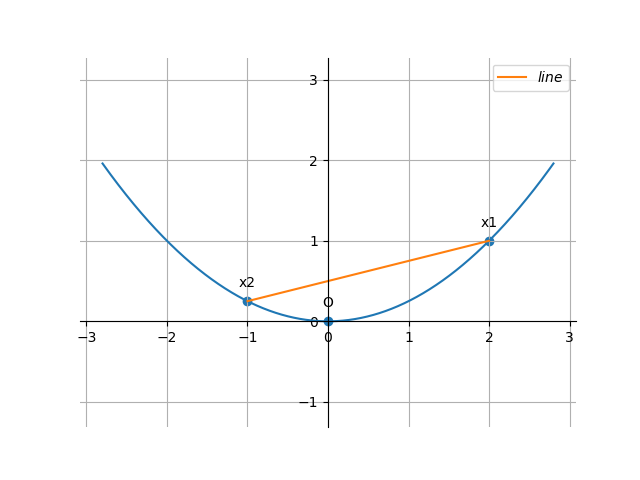
\includegraphics[width=0.75\columnwidth]{conic.png}
\caption{Tangents from A to circle through B, C and D}
\label{fig:triangle}
\end{figure}

The given equation of parabola $x^2 = 4y$ can be written in the general quadratic form as
\begin{align}
    \label{eq:conic_quad_form}
    \vec{x}^{\top}\vec{V}\vec{x}+2\vec{u}^{\top}\vec{x}+f=0
    \end{align}
where
\begin{align}
	\label{eq:V_matrix}
	\vec{V} &= \myvec{1 & 0\\0 & 0},
	\\
	\label{eq:u_vector}
	\vec{u} &= \myvec{0\\-2},
	\\
	\label{eq:f_value}
	f &= 0
	%\\
\end{align}

Let the point from which normals are drawn be $\vec{h}$. Then, the equation of the normal can be written as
\begin{align}
	\vec{x} = \vec{h} + \lambda\vec{m}
	\label{eq:normal_chord}
\end{align}
Say the point of intersection of \eqref{eq:normal_chord} with the conic is $\vec{q}$. A tangent drawn at $\vec{q}$ satisfies the equation
\begin{align}
	\label{eq:tangency_condition}
	\vec{n}^\top(\vec{Vq}+\vec{u}) = 0
\end{align}
Where $\vec{n}$ is the direction vector of the tangent and is perpendicular to $\vec{m}$ in \eqref{eq:normal_chord}.\\\\
In general, the parameter values for points of intersection of a line given by \eqref{eq:normal_chord} with a conic is given by
{\tiny
\begin{multline}
\lambda_i = \frac{1}
{
\vec{m}^T\vec{V}\vec{m}
}
\lbrak{-\vec{m}^T\brak{\vec{V}\vec{h}+\vec{u}}}
\\
\pm
\rbrak{\sqrt{
\sbrak{
\vec{m}^T\brak{\vec{V}\vec{h}+\vec{u}}
}^2
-
\brak
{
\vec{h}^T\vec{V}\vec{h} + 2\vec{u}^T\vec{h} +f
}
\brak{\vec{m}^T\vec{V}\vec{m}}
}
}
\label{eq:tangent_roots}
\end{multline}
}
Using \eqref{eq:tangent_roots} and \eqref{eq:normal_chord}, the intersection point $\vec{q}$ can be written as
\begin{align}
	\label{eq:point_of_tangency}
	\vec{q} = \vec{h} + \lambda_i\vec{m}
\end{align}
Substituting \eqref{eq:point_of_tangency} in \eqref{eq:tangency_condition},
\begin{align}
	\label{eq:normal_simp_1}
	\vec{n}^\top(\vec{V}(\vec{h}+\lambda_i\vec{m})+\vec{u}) = 0\\
	\label{eq:normal_simp_2}
	\implies \lambda_i\vec{n}^\top\vec{V}\vec{m} = -\vec{n}^\top(\vec{Vh}+\vec{u})
\end{align}
Substituting value of $\lambda_i$ from \eqref{eq:tangent_roots} in \eqref{eq:normal_simp_2}
{\tiny
\begin{multline}
	\frac{1}{\vec{m}^\top\vec{V}\vec{m}}\lbrak{-\vec{m}^\top\brak{\vec{Vh}+\vec{u}}} \\ 
	\pm \rbrak{\sqrt{\sbrak{\vec{m}^T\brak{\vec{V}\vec{h}+\vec{u}}}^2-\brak{\vec{h}^T\vec{V}\vec{h} + 2\vec{u}^T\vec{h} +f}\brak{\vec{m}^T\vec{V}\vec{m}}}}\vec{n}^\top\vec{V}\vec{m} \\
	= -\vec{n}^\top\brak{\vec{Vh}+\vec{u}}
	\label{eq:normal_simp_3}
\end{multline}
}
Rearranging the terms,
{\tiny
\begin{multline}
	\pm \sqrt{\sbrak{\vec{m}^T\brak{\vec{V}\vec{h}+\vec{u}}}^2-\brak{\vec{h}^T\vec{V}\vec{h} + 2\vec{u}^T\vec{h} +f}\brak{\vec{m}^T\vec{V}\vec{m}}} \brak{\vec{n}^\top\vec{V}\vec{m}} \\ = \brak{\vec{Vh}+\vec{u}}^\top\brak{\brak{\vec{n}^\top\vec{V}\vec{m}}\vec{m}-\brak{\vec{m}^\top\vec{V}\vec{m}}\vec{n}}
\end{multline}
}
Squaring on both sides
{\tiny
\begin{multline}
	\sbrak{\sbrak{\vec{m}^T\brak{\vec{V}\vec{h}+\vec{u}}}^2-\brak{\vec{h}^T\vec{V}\vec{h} + 2\vec{u}^T\vec{h} +f}\brak{\vec{m}^T\vec{V}\vec{m}}}\brak{\vec{n}^\top\vec{V}\vec{m}}^2 \\ = \sbrak{\brak{\vec{Vh}+\vec{u}}^\top\brak{\brak{\vec{n}^\top\vec{V}\vec{m}}\vec{m}-\brak{\vec{m}^\top\vec{V}\vec{m}}\vec{n}}}^2
	\label{eq:normal_solution}
\end{multline}
}\\
If $\vec{n}$ is taken as $\myvec{-\mu \\ 1}$, then $\vec{m}$ is $\myvec{-1 \\ -\mu}$. Substituting these values in \eqref{eq:normal_solution} and solving for $\mu$, the different possible normals passing through $\vec{h}$ are obtained.\\\\
Thus after solving we get the following values for $\mu$ = {-1, 1/2 - sqrt(3)*I/2, 1/2 + sqrt(3)*I/2}\\\\
Taking $\mu$=1 we get,
\begin{center}
$\vec{n} = \myvec{1 \\ 1}$, $\vec{m} = \myvec{-1 \\ 1}$\\
\end{center}
By calculating $\lambda_i$ from \eqref{eq:normal_simp_2}, we get
\begin{center}
    $\lambda_i = -1$
\end{center}
We find out $\vec{q}$ from \eqref{eq:point_of_tangency},
\begin{center}
where $\vec{h} = \myvec{1 \\ 2}$, $\vec{m} = \myvec{-1 \\ 1}$, $\lambda_i = -1$
\end{center}
\begin{center}
    $\vec{q} = \myvec{1 \\ 2} + (-1)\myvec{-1 \\ 1} = $\myvec{2 \\ 1}
\end{center}
\begin{center}
    Thus $\vec{q}$ satisfies Option(a) i.e. $x+y=3$
\end{center} 

\section*{\large Construction}
{
\setlength\extrarowheight{5pt}
\begin{tabular}{|c|c|c|}
	\hline
	\textbf{Symbol}&\textbf{Value}&\textbf{Description}\\[5pt]
	\hline
	$\vec{h}$&$\myvec{1 \\ 2}$&Given point through which Normal is passing\\[5pt]
	\hline
	$\vec{q}$&$\myvec{2 \\ 1}$&Foot of Normal\\[5pt]
	\hline
	$\vec{m}$ & $\myvec{-1 \\ 1}$ & Direction Vector of Normal\\[5pt]
	\hline
	$\vec{n}$ & $\myvec{1 \\ 1}$ & Direction Vector of Tangent at $\myvec{q}$\\
	\hline
\end{tabular}
}

\end{document}
\fi

\item 
 The line $y=mx+1$ is a tangent to the curve $y^2 = 4x$, find the value of $m$. 
 \\
 \solution 
\label{chapters/12/6/6/21}
\iffalse
\documentclass[journal,10pt,twocolumn]{article}
\usepackage{graphicx, float}
\usepackage[margin=0.5in]{geometry}
\usepackage{amsmath, bm}
\usepackage{array}
\usepackage{booktabs}
\usepackage[utf8]{inputenc}
\usepackage{amsfonts}
\usepackage{amssymb}
\usepackage{graphicx}
\usepackage{multicol}
\usepackage{tabularx}
\usepackage{hyperref}
\usepackage{mathtools}
\DeclareUnicodeCharacter{2212}{-}
\providecommand{\norm}[1]{\left\lVert#1\right\rVert}
\providecommand{\abs}[1]{\left\vert#1\right\vert}
\let\vec\mathbf
\newcommand{\myvec}[1]{\ensuremath{\begin{pmatrix}#1\end{pmatrix}}}
\newcommand{\mydet}[1]{\ensuremath{\begin{vmatrix}#1\end{vmatrix}}}
\providecommand{\brak}[1]{\ensuremath{\left(#1\right)}}
\providecommand{\lbrak}[1]{\ensuremath{\left(#1\right.}}
\providecommand{\rbrak}[1]{\ensuremath{\left.#1\right)}}
\providecommand{\sbrak}[1]{\ensuremath{{}\left[#1\right]}}
%\providecommand{\norm}[1]{\left\lVert#1\right\rVert}
%\providecommand{\sbrak}[1]{\ensuremath{{}\left[#1\right]}}
%\providecommand{\lsbrak}[1]{\ensuremath{{}\left[#1\right.}}
%\providecommand{\rsbrak}[1]{\ensuremath{{}\left.#1\right]}}
%\providecommand{\brak}[1]{\ensuremath{\left(#1\right)}}
%\providecommand{\lbrak}[1]{\ensuremath{\left(#1\right.}}
%\providecommand{\rbrak}[1]{\ensuremath{\left.#1\right)}}
%\providecommand{\cbrak}[1]{\ensuremath{\left\{#1\right\}}}
%\providecommand{\lcbrak}[1]{\ensuremath{\left\{#1\right.}}
%\providecommand{\rcbrak}[1]{\ensuremath{\left.#1\right\}}}
%\newcommand{\myvec}[1]{\ensuremath{\begin{pmatrix}#1\end{pmatrix}}}
%\let\vec\mathbf

\title{\textbf{Conic Assignment}}
\author{Namrath Pinnamaneni \hspace{9cm} FWC22042}
\date{September 2022}

\begin{document}

\maketitle
\paragraph{\textit{Problem Statement} -
\fi
Find the normal to the curve $x_2=4y$ passing (1,2). 
\iffalse
(a)x+y=3  \hspace{2cm} (b)x-y=3\\ 
(c)x+y=1 \hspace{2cm}  (d)x-y=1\\}

\section*{\large Solution}

\begin{figure}[H]
\centering
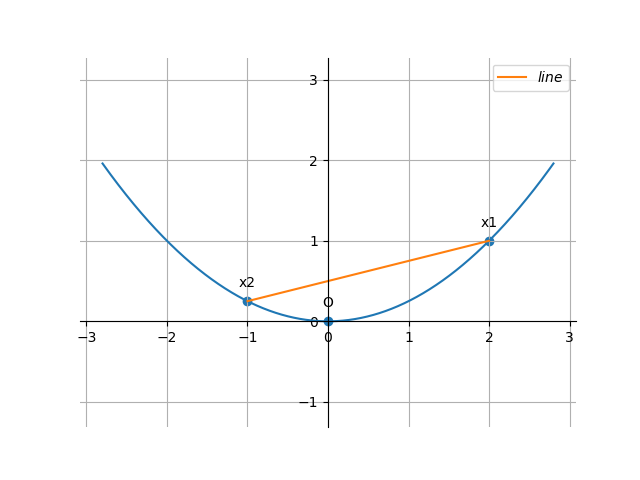
\includegraphics[width=0.75\columnwidth]{conic.png}
\caption{Tangents from A to circle through B, C and D}
\label{fig:triangle}
\end{figure}

The given equation of parabola $x^2 = 4y$ can be written in the general quadratic form as
\begin{align}
    \label{eq:conic_quad_form}
    \vec{x}^{\top}\vec{V}\vec{x}+2\vec{u}^{\top}\vec{x}+f=0
    \end{align}
where
\begin{align}
	\label{eq:V_matrix}
	\vec{V} &= \myvec{1 & 0\\0 & 0},
	\\
	\label{eq:u_vector}
	\vec{u} &= \myvec{0\\-2},
	\\
	\label{eq:f_value}
	f &= 0
	%\\
\end{align}

Let the point from which normals are drawn be $\vec{h}$. Then, the equation of the normal can be written as
\begin{align}
	\vec{x} = \vec{h} + \lambda\vec{m}
	\label{eq:normal_chord}
\end{align}
Say the point of intersection of \eqref{eq:normal_chord} with the conic is $\vec{q}$. A tangent drawn at $\vec{q}$ satisfies the equation
\begin{align}
	\label{eq:tangency_condition}
	\vec{n}^\top(\vec{Vq}+\vec{u}) = 0
\end{align}
Where $\vec{n}$ is the direction vector of the tangent and is perpendicular to $\vec{m}$ in \eqref{eq:normal_chord}.\\\\
In general, the parameter values for points of intersection of a line given by \eqref{eq:normal_chord} with a conic is given by
{\tiny
\begin{multline}
\lambda_i = \frac{1}
{
\vec{m}^T\vec{V}\vec{m}
}
\lbrak{-\vec{m}^T\brak{\vec{V}\vec{h}+\vec{u}}}
\\
\pm
\rbrak{\sqrt{
\sbrak{
\vec{m}^T\brak{\vec{V}\vec{h}+\vec{u}}
}^2
-
\brak
{
\vec{h}^T\vec{V}\vec{h} + 2\vec{u}^T\vec{h} +f
}
\brak{\vec{m}^T\vec{V}\vec{m}}
}
}
\label{eq:tangent_roots}
\end{multline}
}
Using \eqref{eq:tangent_roots} and \eqref{eq:normal_chord}, the intersection point $\vec{q}$ can be written as
\begin{align}
	\label{eq:point_of_tangency}
	\vec{q} = \vec{h} + \lambda_i\vec{m}
\end{align}
Substituting \eqref{eq:point_of_tangency} in \eqref{eq:tangency_condition},
\begin{align}
	\label{eq:normal_simp_1}
	\vec{n}^\top(\vec{V}(\vec{h}+\lambda_i\vec{m})+\vec{u}) = 0\\
	\label{eq:normal_simp_2}
	\implies \lambda_i\vec{n}^\top\vec{V}\vec{m} = -\vec{n}^\top(\vec{Vh}+\vec{u})
\end{align}
Substituting value of $\lambda_i$ from \eqref{eq:tangent_roots} in \eqref{eq:normal_simp_2}
{\tiny
\begin{multline}
	\frac{1}{\vec{m}^\top\vec{V}\vec{m}}\lbrak{-\vec{m}^\top\brak{\vec{Vh}+\vec{u}}} \\ 
	\pm \rbrak{\sqrt{\sbrak{\vec{m}^T\brak{\vec{V}\vec{h}+\vec{u}}}^2-\brak{\vec{h}^T\vec{V}\vec{h} + 2\vec{u}^T\vec{h} +f}\brak{\vec{m}^T\vec{V}\vec{m}}}}\vec{n}^\top\vec{V}\vec{m} \\
	= -\vec{n}^\top\brak{\vec{Vh}+\vec{u}}
	\label{eq:normal_simp_3}
\end{multline}
}
Rearranging the terms,
{\tiny
\begin{multline}
	\pm \sqrt{\sbrak{\vec{m}^T\brak{\vec{V}\vec{h}+\vec{u}}}^2-\brak{\vec{h}^T\vec{V}\vec{h} + 2\vec{u}^T\vec{h} +f}\brak{\vec{m}^T\vec{V}\vec{m}}} \brak{\vec{n}^\top\vec{V}\vec{m}} \\ = \brak{\vec{Vh}+\vec{u}}^\top\brak{\brak{\vec{n}^\top\vec{V}\vec{m}}\vec{m}-\brak{\vec{m}^\top\vec{V}\vec{m}}\vec{n}}
\end{multline}
}
Squaring on both sides
{\tiny
\begin{multline}
	\sbrak{\sbrak{\vec{m}^T\brak{\vec{V}\vec{h}+\vec{u}}}^2-\brak{\vec{h}^T\vec{V}\vec{h} + 2\vec{u}^T\vec{h} +f}\brak{\vec{m}^T\vec{V}\vec{m}}}\brak{\vec{n}^\top\vec{V}\vec{m}}^2 \\ = \sbrak{\brak{\vec{Vh}+\vec{u}}^\top\brak{\brak{\vec{n}^\top\vec{V}\vec{m}}\vec{m}-\brak{\vec{m}^\top\vec{V}\vec{m}}\vec{n}}}^2
	\label{eq:normal_solution}
\end{multline}
}\\
If $\vec{n}$ is taken as $\myvec{-\mu \\ 1}$, then $\vec{m}$ is $\myvec{-1 \\ -\mu}$. Substituting these values in \eqref{eq:normal_solution} and solving for $\mu$, the different possible normals passing through $\vec{h}$ are obtained.\\\\
Thus after solving we get the following values for $\mu$ = {-1, 1/2 - sqrt(3)*I/2, 1/2 + sqrt(3)*I/2}\\\\
Taking $\mu$=1 we get,
\begin{center}
$\vec{n} = \myvec{1 \\ 1}$, $\vec{m} = \myvec{-1 \\ 1}$\\
\end{center}
By calculating $\lambda_i$ from \eqref{eq:normal_simp_2}, we get
\begin{center}
    $\lambda_i = -1$
\end{center}
We find out $\vec{q}$ from \eqref{eq:point_of_tangency},
\begin{center}
where $\vec{h} = \myvec{1 \\ 2}$, $\vec{m} = \myvec{-1 \\ 1}$, $\lambda_i = -1$
\end{center}
\begin{center}
    $\vec{q} = \myvec{1 \\ 2} + (-1)\myvec{-1 \\ 1} = $\myvec{2 \\ 1}
\end{center}
\begin{center}
    Thus $\vec{q}$ satisfies Option(a) i.e. $x+y=3$
\end{center} 

\section*{\large Construction}
{
\setlength\extrarowheight{5pt}
\begin{tabular}{|c|c|c|}
	\hline
	\textbf{Symbol}&\textbf{Value}&\textbf{Description}\\[5pt]
	\hline
	$\vec{h}$&$\myvec{1 \\ 2}$&Given point through which Normal is passing\\[5pt]
	\hline
	$\vec{q}$&$\myvec{2 \\ 1}$&Foot of Normal\\[5pt]
	\hline
	$\vec{m}$ & $\myvec{-1 \\ 1}$ & Direction Vector of Normal\\[5pt]
	\hline
	$\vec{n}$ & $\myvec{1 \\ 1}$ & Direction Vector of Tangent at $\myvec{q}$\\
	\hline
\end{tabular}
}

\end{document}
\fi

\item 
\label{chapters/12/6/6/22}
Find the normal at the point (1,1) on the curve 
\begin{align}
2y+x^2=3
\end{align}
\solution
\iffalse
\documentclass[journal,10pt,twocolumn]{article}
\usepackage{graphicx, float}
\usepackage[margin=0.5in]{geometry}
\usepackage{amsmath, bm}
\usepackage{array}
\usepackage{booktabs}
\usepackage[utf8]{inputenc}
\usepackage{amsfonts}
\usepackage{amssymb}
\usepackage{graphicx}
\usepackage{multicol}
\usepackage{tabularx}
\usepackage{hyperref}
\usepackage{mathtools}
\DeclareUnicodeCharacter{2212}{-}
\providecommand{\norm}[1]{\left\lVert#1\right\rVert}
\providecommand{\abs}[1]{\left\vert#1\right\vert}
\let\vec\mathbf
\newcommand{\myvec}[1]{\ensuremath{\begin{pmatrix}#1\end{pmatrix}}}
\newcommand{\mydet}[1]{\ensuremath{\begin{vmatrix}#1\end{vmatrix}}}
\providecommand{\brak}[1]{\ensuremath{\left(#1\right)}}
\providecommand{\lbrak}[1]{\ensuremath{\left(#1\right.}}
\providecommand{\rbrak}[1]{\ensuremath{\left.#1\right)}}
\providecommand{\sbrak}[1]{\ensuremath{{}\left[#1\right]}}
%\providecommand{\norm}[1]{\left\lVert#1\right\rVert}
%\providecommand{\sbrak}[1]{\ensuremath{{}\left[#1\right]}}
%\providecommand{\lsbrak}[1]{\ensuremath{{}\left[#1\right.}}
%\providecommand{\rsbrak}[1]{\ensuremath{{}\left.#1\right]}}
%\providecommand{\brak}[1]{\ensuremath{\left(#1\right)}}
%\providecommand{\lbrak}[1]{\ensuremath{\left(#1\right.}}
%\providecommand{\rbrak}[1]{\ensuremath{\left.#1\right)}}
%\providecommand{\cbrak}[1]{\ensuremath{\left\{#1\right\}}}
%\providecommand{\lcbrak}[1]{\ensuremath{\left\{#1\right.}}
%\providecommand{\rcbrak}[1]{\ensuremath{\left.#1\right\}}}
%\newcommand{\myvec}[1]{\ensuremath{\begin{pmatrix}#1\end{pmatrix}}}
%\let\vec\mathbf

\title{\textbf{Conic Assignment}}
\author{Namrath Pinnamaneni \hspace{9cm} FWC22042}
\date{September 2022}

\begin{document}

\maketitle
\paragraph{\textit{Problem Statement} -
\fi
Find the normal to the curve $x_2=4y$ passing (1,2). 
\iffalse
(a)x+y=3  \hspace{2cm} (b)x-y=3\\ 
(c)x+y=1 \hspace{2cm}  (d)x-y=1\\}

\section*{\large Solution}

\begin{figure}[H]
\centering
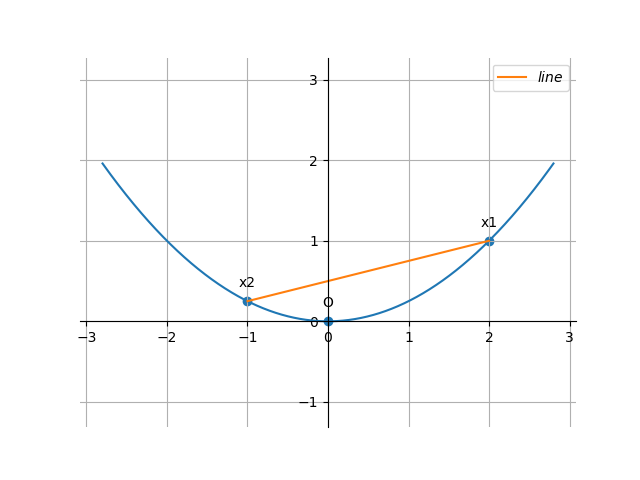
\includegraphics[width=0.75\columnwidth]{conic.png}
\caption{Tangents from A to circle through B, C and D}
\label{fig:triangle}
\end{figure}

The given equation of parabola $x^2 = 4y$ can be written in the general quadratic form as
\begin{align}
    \label{eq:conic_quad_form}
    \vec{x}^{\top}\vec{V}\vec{x}+2\vec{u}^{\top}\vec{x}+f=0
    \end{align}
where
\begin{align}
	\label{eq:V_matrix}
	\vec{V} &= \myvec{1 & 0\\0 & 0},
	\\
	\label{eq:u_vector}
	\vec{u} &= \myvec{0\\-2},
	\\
	\label{eq:f_value}
	f &= 0
	%\\
\end{align}

Let the point from which normals are drawn be $\vec{h}$. Then, the equation of the normal can be written as
\begin{align}
	\vec{x} = \vec{h} + \lambda\vec{m}
	\label{eq:normal_chord}
\end{align}
Say the point of intersection of \eqref{eq:normal_chord} with the conic is $\vec{q}$. A tangent drawn at $\vec{q}$ satisfies the equation
\begin{align}
	\label{eq:tangency_condition}
	\vec{n}^\top(\vec{Vq}+\vec{u}) = 0
\end{align}
Where $\vec{n}$ is the direction vector of the tangent and is perpendicular to $\vec{m}$ in \eqref{eq:normal_chord}.\\\\
In general, the parameter values for points of intersection of a line given by \eqref{eq:normal_chord} with a conic is given by
{\tiny
\begin{multline}
\lambda_i = \frac{1}
{
\vec{m}^T\vec{V}\vec{m}
}
\lbrak{-\vec{m}^T\brak{\vec{V}\vec{h}+\vec{u}}}
\\
\pm
\rbrak{\sqrt{
\sbrak{
\vec{m}^T\brak{\vec{V}\vec{h}+\vec{u}}
}^2
-
\brak
{
\vec{h}^T\vec{V}\vec{h} + 2\vec{u}^T\vec{h} +f
}
\brak{\vec{m}^T\vec{V}\vec{m}}
}
}
\label{eq:tangent_roots}
\end{multline}
}
Using \eqref{eq:tangent_roots} and \eqref{eq:normal_chord}, the intersection point $\vec{q}$ can be written as
\begin{align}
	\label{eq:point_of_tangency}
	\vec{q} = \vec{h} + \lambda_i\vec{m}
\end{align}
Substituting \eqref{eq:point_of_tangency} in \eqref{eq:tangency_condition},
\begin{align}
	\label{eq:normal_simp_1}
	\vec{n}^\top(\vec{V}(\vec{h}+\lambda_i\vec{m})+\vec{u}) = 0\\
	\label{eq:normal_simp_2}
	\implies \lambda_i\vec{n}^\top\vec{V}\vec{m} = -\vec{n}^\top(\vec{Vh}+\vec{u})
\end{align}
Substituting value of $\lambda_i$ from \eqref{eq:tangent_roots} in \eqref{eq:normal_simp_2}
{\tiny
\begin{multline}
	\frac{1}{\vec{m}^\top\vec{V}\vec{m}}\lbrak{-\vec{m}^\top\brak{\vec{Vh}+\vec{u}}} \\ 
	\pm \rbrak{\sqrt{\sbrak{\vec{m}^T\brak{\vec{V}\vec{h}+\vec{u}}}^2-\brak{\vec{h}^T\vec{V}\vec{h} + 2\vec{u}^T\vec{h} +f}\brak{\vec{m}^T\vec{V}\vec{m}}}}\vec{n}^\top\vec{V}\vec{m} \\
	= -\vec{n}^\top\brak{\vec{Vh}+\vec{u}}
	\label{eq:normal_simp_3}
\end{multline}
}
Rearranging the terms,
{\tiny
\begin{multline}
	\pm \sqrt{\sbrak{\vec{m}^T\brak{\vec{V}\vec{h}+\vec{u}}}^2-\brak{\vec{h}^T\vec{V}\vec{h} + 2\vec{u}^T\vec{h} +f}\brak{\vec{m}^T\vec{V}\vec{m}}} \brak{\vec{n}^\top\vec{V}\vec{m}} \\ = \brak{\vec{Vh}+\vec{u}}^\top\brak{\brak{\vec{n}^\top\vec{V}\vec{m}}\vec{m}-\brak{\vec{m}^\top\vec{V}\vec{m}}\vec{n}}
\end{multline}
}
Squaring on both sides
{\tiny
\begin{multline}
	\sbrak{\sbrak{\vec{m}^T\brak{\vec{V}\vec{h}+\vec{u}}}^2-\brak{\vec{h}^T\vec{V}\vec{h} + 2\vec{u}^T\vec{h} +f}\brak{\vec{m}^T\vec{V}\vec{m}}}\brak{\vec{n}^\top\vec{V}\vec{m}}^2 \\ = \sbrak{\brak{\vec{Vh}+\vec{u}}^\top\brak{\brak{\vec{n}^\top\vec{V}\vec{m}}\vec{m}-\brak{\vec{m}^\top\vec{V}\vec{m}}\vec{n}}}^2
	\label{eq:normal_solution}
\end{multline}
}\\
If $\vec{n}$ is taken as $\myvec{-\mu \\ 1}$, then $\vec{m}$ is $\myvec{-1 \\ -\mu}$. Substituting these values in \eqref{eq:normal_solution} and solving for $\mu$, the different possible normals passing through $\vec{h}$ are obtained.\\\\
Thus after solving we get the following values for $\mu$ = {-1, 1/2 - sqrt(3)*I/2, 1/2 + sqrt(3)*I/2}\\\\
Taking $\mu$=1 we get,
\begin{center}
$\vec{n} = \myvec{1 \\ 1}$, $\vec{m} = \myvec{-1 \\ 1}$\\
\end{center}
By calculating $\lambda_i$ from \eqref{eq:normal_simp_2}, we get
\begin{center}
    $\lambda_i = -1$
\end{center}
We find out $\vec{q}$ from \eqref{eq:point_of_tangency},
\begin{center}
where $\vec{h} = \myvec{1 \\ 2}$, $\vec{m} = \myvec{-1 \\ 1}$, $\lambda_i = -1$
\end{center}
\begin{center}
    $\vec{q} = \myvec{1 \\ 2} + (-1)\myvec{-1 \\ 1} = $\myvec{2 \\ 1}
\end{center}
\begin{center}
    Thus $\vec{q}$ satisfies Option(a) i.e. $x+y=3$
\end{center} 

\section*{\large Construction}
{
\setlength\extrarowheight{5pt}
\begin{tabular}{|c|c|c|}
	\hline
	\textbf{Symbol}&\textbf{Value}&\textbf{Description}\\[5pt]
	\hline
	$\vec{h}$&$\myvec{1 \\ 2}$&Given point through which Normal is passing\\[5pt]
	\hline
	$\vec{q}$&$\myvec{2 \\ 1}$&Foot of Normal\\[5pt]
	\hline
	$\vec{m}$ & $\myvec{-1 \\ 1}$ & Direction Vector of Normal\\[5pt]
	\hline
	$\vec{n}$ & $\myvec{1 \\ 1}$ & Direction Vector of Tangent at $\myvec{q}$\\
	\hline
\end{tabular}
}

\end{document}
\fi

 \item If the line $y=\sqrt{3}x+K$ touches the parabola $x^2=16y,$ then find the value of $K$.
\item If the line $y=mx+1$ is tangent to the parabola $y^2=4x$ then find the value of $m$.
\item Find the condition that the curves $2x=y^2$ and $2xy=k$ intersect orthogonally.
\item Prove that the curves $xy=4$ and $x^2+y^2=8$ touch each other.
\item Find the angle of intersection of the curves $y=4-x^2$ and $y=x^2$.
\item Prove that the curves $y^2=4x$ and $x^2+y^2-6x+1=0$ touch each each other at the point (1,2).
\item Find the equation of the normal lines to the curve $3x^2-y^2=8$ which are parallel to the line $x+3y=4$.
 \item The equation of the normal to the curve $3x^2-y^2 =8$ which is parallel to the line $x+3y=8$ is
 \begin{enumerate}
 \item $3x-y=8$
 \item $3x+y+8=0$
 \item $x+3y+8=0$
 \item $x+3y=0$
 \end{enumerate}
\item The equation of the tangent to the curve $(1+y^2) =2-x$, where it crosses the x-axis is 
\begin{enumerate}
\item $x+5y=2$
\item $x-5y=2$
\item $5x-y=2$
\item $5x+y=2$
\end{enumerate}
\end{enumerate}
State whether the statements are True or False 
\begin{enumerate}[label=\thesection.\arabic*,ref=\thesection.\theenumi,resume*]
\item The line $lx+my+n=0$ will touch the parabola $y^2=4 ax$ if $ln =am^2$,
\item The line $2x+3y=12$ touches the ellipse $\frac{x^2}{9}+\frac{y^2}{4}=2$ at the point (3,2).
\end{enumerate}
